\documentclass[10pt]{article}
\usepackage[T1]{fontenc}
\usepackage[utf8]{inputenc}
\usepackage[nottoc]{tocbibind}
\usepackage{graphicx}
\usepackage{indentfirst}
\usepackage[margin=0.8in]{geometry}
\usepackage{hyperref}
\usepackage{float}
\usepackage[polish]{babel}
\usepackage[sorting=none]{biblatex}
\usepackage{csquotes}
\usepackage{amsfonts}
\usepackage{amsmath}
\usepackage{caption}
\usepackage{subcaption}

\graphicspath{{./images/}}
\addbibresource{bibliography.bib}

\title{Badanie możliwości rozwiązania problemu CVRP z użyciem algorytmu mrówkowego\\
\large{Raport}}
\author{Szymon Stasiak}
\date{\today}

\begin{document}

\maketitle
\begin{abstract}
Oparty na problemie komiwojażera, problem CVRP jest problemem, dla którego dokładnego rozwiązania nie da się uzyskać w wyniku działania algorytmu o złożoności wielomianowej. Jako, iż temat ten często pojawia się w sytuacjach takich jak planowanie tras kurierów w firmach dostawczych, ciągle trwają próby stworzenia kolejnych algorytmów, oferujących coraz to dokładniejsze przybliżenia. Dokument ten przedstawia wykorzystanie do rozwiązania tego problemu znanej metaheurystyki z dziedziny sztucznej inteligencji - optymalizacji kolonią mrówek.

Porównane zostały trzy znane w literaturze warianty optymalizacji tego problemu: wersja podstawowa w formie zaprezentowanej pod koniec XX wieku oraz ulepszenia dodające mrówki elitarne a także modyfikujące lokalnie znalezione rozwiązanie poprzez odwracanie części ścieżek. Badania przeprowadzone na wielokrotnie analizowanych zbiorach testowych, zawierających od 32 do 60 odbiorców, wykazały znaczną przewagę zastosowanej metaheurystyki w odniesienia do podejścia heurystycznego.

Wzajemnie porównane zostały również wszystkie trzy warianty zaimplementowanego podejścia. W wyniku badań dla pięciu testowych instancji, obie modyfikacje podstawowej wersji okazały się poprawiać znajdowane rozwiązania. W przypadku wariantu z mrówkami elitarnymi poprawa ta nastąpiła bez wpływu na czas działania algorytmu. Drugi z wariantów z kolei, wymagając dłuższego czasu działania, w niektórych przypadkach pozwolił osiągnąć kilkukrotną minimalizację błędu względem oczekiwanego rozwiązania.

Przedstawiony dokument zawiera również dokładny opis procesu wyboru parametrów wpływających na optymalne działanie wszystkich wariantów optymalizacji kolonią mrówek zaimplementowanych dla rozwiązywanego problemu. W procesie tym zbadany został wpływ kluczowych współczynników na zachowanie algorytmów, a co za tym idzie, na jakość znalezionego rozwiązania i szybkość jego wyznaczenia.
\end{abstract}

\newpage
\tableofcontents
\newpage

\section{Opis problemu}
\label{sec:problem}
\textbf{Problem CVRP~\cite{Dorigo2004}} (\textit{Capacitated Vehicle Routing Problem}) dotyczy znajdowania optymalnego rozkładu tras dla floty ciężarówek mającej dostarczyć towar z centralnego magazynu do znajdujących się w określonych lokalizacjach odbiorców. Lokalizacje każdej pary odbiorców połączone są ze sobą za pomocą dróg o długości będącej odległością euklidesową pomiędzy lokalizacjami odbiorców. Przez \textquote{optymalny rozkład tras} rozumie się zestaw tras o najmniejszej sumarycznej długości taki, że:
\begin{itemize}
    \item Każda trasa zaczyna i kończy się w magazynie centralnym.
    \item Każdy z odbiorców jest odwiedzony przez dokładnie jedną ciężarówkę, która dostarcza mu ilość towaru równą z góry określonemu zapotrzebowaniu tego odbiorcy. Po odwiedzeniu odbiorcy, ilość towaru w ciężarówce ulega zmniejszeniu o ilość dostarczoną.
    \item Każda ciężarówka ma jednakową, z góry określoną, maksymalną sumaryczną ilość towaru którą może dostarczyć.
\end{itemize}

W zakresie tego projektu analizowana będzie zmodyfikowana wersja problemu CVRP, gdzie maksymalna droga którą może przebyć pojedynczy pojazd podana jest na wejściu, podobnie jak liczba pojazdów.

\subsection{Ujęcie algorytmiczne}
W algorytmicznym rozumieniu problemu, powyższe informacje można przedstawić jako zestaw danych:
\begin{itemize}
    \item $n$ - liczba odbiorców
    \item $G(V,E,d)$ - ważony graf pełny nieskierowany o wierzchołkach ze zbioru $V = \{v_0,v_1,\dots,v_n\}$, gdzie $v_0$ oznacza magazyn centralny, zaś pozostałe wierzchołki to odbiorcy. Każdy z wierzchołków w $V$ ma przypisane współrzędne na płaszczyźnie. $E$ jest zbiorem krawędzi, zaś $d$ to funkcja wagi krawędzi $d: E \rightarrow \mathbb{R}$ o wartości równej odległości euklidesowej między dwoma wierzchołkami łączonymi przez daną krawędź
    \item $(q_1,\ldots,q_n)$ - ciąg $n$ liczb całkowitych oznaczających zapotrzebowanie kolejnych odbiorców
    \item $m$ - liczba ciężarówek
    \item $Q$ - maksymalna sumaryczna ilość towaru którą może dostarczyć pojedyncza ciężarówka
    \item $s_{max}$ - maksymalna droga którą może przebyć pojedynczy pojazd
\end{itemize}
Na wyjściu oczekiwane są trasy dla wszystkich pojazdów (tj. $m$ ciągów postaci $(0=i_1^{j}, i_2^{j}, \dots, i_k^{j}=0)$, gdzie $i_l^{j}$ oznacza indeks wierzchołka grafu odwiedzonego jako $l$-ty w kolejności na trasie $j$-tego pojazdu) oraz sumaryczna długość tych tras.

\section{Algorytm mrówkowy}
Klasyczny algorytm mrówkowy został zaproponowany jako metoda szukania optymalnych dróg w grafach, poprzez przypisanie krawędziom grafów specjalnych wartości (ilości feromonów)~\cite{Dorigo1996}\cite{Dorigo1999}. Wartości te, nadane na podstawie poprzednich iteracji algorytmu, wskazują, które krawędzie mają potencjał dawać finalnie lepsze ścieżki. Ilość feromonów na krawędziach niewybieranych do optymalnych rozwiązań w kolejnych iteracjach spada, zaś na pozostałych rośnie, pozwalając po pewnej liczbie iteracji ustabilizować wybór ścieżki.

Warto wspomnieć, iż algorytm mrówkowy w swojej podstawowej wersji znajduje jedną optymalną ścieżkę, spełniającą określone kryteria budowy. Radzi sobie więc dobrze przykładowo przy rozwiązywaniu problemu komiwojażera. W przypadku CVRP, poszukiwany jest zestaw ścieżek. W tym celu wszystkie wersje zaimplementowanego algorytmu mrówkowego opierać się będą na modyfikacji algorytmu mrówkowego dla wyszukiwania cyklu Hamiltona. Modyfikacja polegać będzie na dopuszczeniu wielokrotnego odwiedzania wierzchołka startowego, przy czym po każdej z takich wizyt przywracana zostaje początkowa ilość towaru w ciężarówce oraz ponownie \textquote{uruchomiany} jest licznik maksymalnej drogi którą może przebyć pojazd. Tak znaleziona ścieżka może zostać na końcu podzielona w miejscu każdego odwiedzenia  wierzchołka startowego, tworząc zestaw ścieżek spełniających wymagania zadania.

W celu dokładniejszej analizy działania algorytmu mrówkowego dla problemu CVRP, porównane zostanie działanie klasycznej wersji tego algorytmu, dwóch wariantów jego modyfikacji oraz algorytmu zachłannego.

\subsection{Wprowadzenie mrówek elitarnych}
Wraz z pierwszym sformułowaniem algorytmu mrówkowego, zaproponowana została pierwsza modyfikacja mająca potencjał poprawić uzyskiwane wyniki - \textbf{elitist strategy~\cite{Dorigo1996}}. Strategia ta modyfikuje podstawową wersję algorytmu dodając określonej liczbie mrówek (tzw. mrówkom elitarnym) możliwość pozostawianie dodatkowej ilości feromonów na dotychczas najlepszej ścieżce. Podejście to, przy odpowiednio dobranym ograniczeniu liczby mrówek elitarnych, ma za zadanie przyspieszenie znalezienia optymalnego rozwiązania.

\subsection{Odwracanie częściowych ścieżek}
Druga z proponowanych modyfikacji również została zaczerpnięta z literatury~\cite{Ayop2020} jako strategia mająca potencjał poprawić wyniki standardowego algorytmu mrówkowego. Jest to jedna z trzech heurystyk przedstawionych we wspomnianej publikacji - odwracanie częściowych ścieżek. Zgodnie z tą heurystyką, po wybraniu ścieżki $P$ dla danej iteracji, składającej się z $k \geq 2$ wierzchołków, odwracane są kolejno wszystkie fragmenty tej ścieżki, ograniczone z obu stron przez wierzchołek będący magazynem centralnym, o wszystkich możliwych długościach od $2$ do $k - 1$. Wybierana jest najbardziej optymalna ze sprawdzonych ścieżek i to ona zostaje uznana za ścieżkę odnalezioną przez daną mrówkę w danej iteracji.

\section{Wyniki eksperymentów}
\label{sec:experiments}
Wszystkie testy w obrębie projektu zostały przeprowadzone na ogólnodostępnych instancjach problemu CVRP pochodzących z pracy~\cite{Augerat1995} i często używanych w pracach poruszających ten problem. Warto nadmienić, iż we wcześniejszych fazach planowano użycie innych zbiorów testowych z innej publikacji, jednak z powodu niedostępności optymalnych wyników oraz wielkości przedstawionych instancji, podjęta została decyzja o zmianie.

Niemniej, aby jeszcze bardziej ujednolicić dane wykorzystywane przez wszystkie testowane algorytmy, występujące w nich parametry zostały wybrane za pomocą eksperymentów wykonywanych na podstawowej implementacji algorytmu mrówkowego. Do tych parametrów należą:
\begin{itemize}
    \item $N$ - liczby mrówek - wykorzystywana wyłącznie w algorytmach mrówkowych
    \item $M$ - maksymalna liczba iteracji - wykorzystywana wyłącznie w algorytmach mrówkowych
    \item $\alpha$ i $\beta$ - współczynniki regulujące wpływ feromonów oraz podejścia heurystycznego przy wyborze kolejnych miast
    \item $\rho$ - współczynnik parowania feromonu
    \item $Q$ - mnożnik dodawanej wartości feromonów
\end{itemize}

Kolejne sekcje opisują w dokładniejszy sposób przebieg eksperymentów mających na celu ustalenie wartości tych współczynników. Opierając się w sporej części na publikacjach źródłowych~\cite{Dorigo1996}\cite{Dorigo1999}, przyjęto następujące domyślne wartości parametrów (używane w testach przed wybraniem nowych współczynników):
\begin{itemize}
    \item $M = 1000$
    \item $\alpha = 1$ i $\beta = 5$
    \item $\rho = 0.5$
    \item $Q = 1$
    \item $s_{max} = 300$
\end{itemize}

O ile nie podano inaczej, wyznaczanie parametrów przeprowadzono poprzez realizację algorytmu mrówkowego na trzech zbiorach testowych: \textit{A-n32-k5}, \textit{A-n45-k7}, \textit{A-n60-k9}, powtarzając wykonanie każdego testu pięciokrotnie, dla różnych wartości ziarna: \textit{11174}, \textit{203019}, \textit{473}, \textit{22087} oraz \textit{121769}.

\subsection{Wybór liczby mrówek $N$ i liczby iteracji $M$}
Analiza wyników opisanych w cytowanych publikacjach pozwala wysnuć hipotezę o wpływie ilości mrówek zarówno na jakość otrzymanych wyników, jak i szybkość zbieżności metody. Z tego też powodu pierwsza grupa testów ma na celu sprawdzenie błędów względnych uzyskanych wyników, a także dynamiki zmiany wyników w kolejnych iteracjach, w zależności od przyjętej liczby mrówek.

W celu lepszego dopasowania do różnych rozmiarów zbiorów testowych, zdecydowano się na uzależnienie liczby mrówek od liczby odbiorców w danym zbiorze testowym. Tak też, dla danej liczby odbiorców $n$, porównano wyniki dla $N \in \left\{ \left\lfloor\frac{n}{8}\right\rfloor, \left\lfloor\frac{n}{4}\right\rfloor, \left\lfloor\frac{n}{3}\right\rfloor, \left\lfloor\frac{n}{2}\right\rfloor, n \right\}$.

W celu określenia jakości znalezionego rozwiązania w kolejnych przypadkach, zestawiono średnią wartość błędu względnego pomiędzy rozwiązaniem znalezionym a rozwiązaniem optymalnym oraz odchylenie standardowe dla różnych wartości ziarna. Wartości te, w zależności od ilości mrówek i zbioru testowego przedstawiają poniższe rysunki \ref{fig:errors} oraz \ref{fig:deviation}. 

\begin{figure}[H]
    \centering
    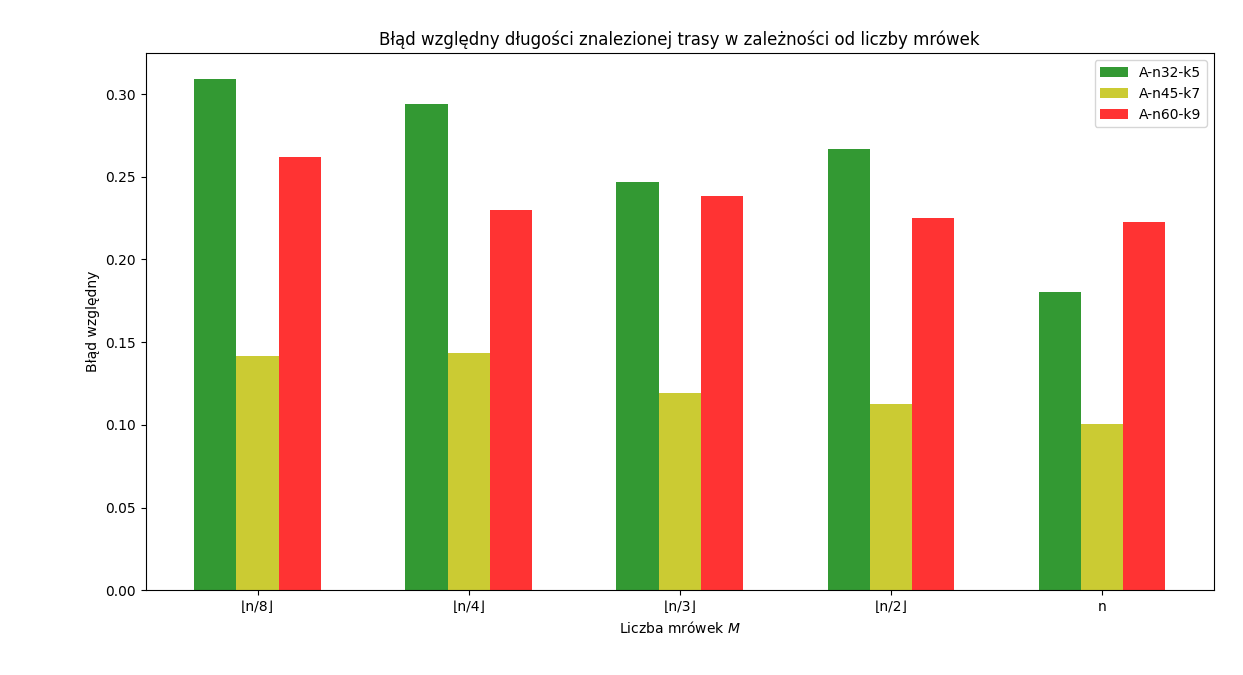
\includegraphics[width=0.75\textwidth]{errors.png}
    \caption{Średni błąd względny długości znalezionych tras w zależności od liczby mrówek}
    \label{fig:errors}
\end{figure}

\begin{figure}[H]
    \centering
    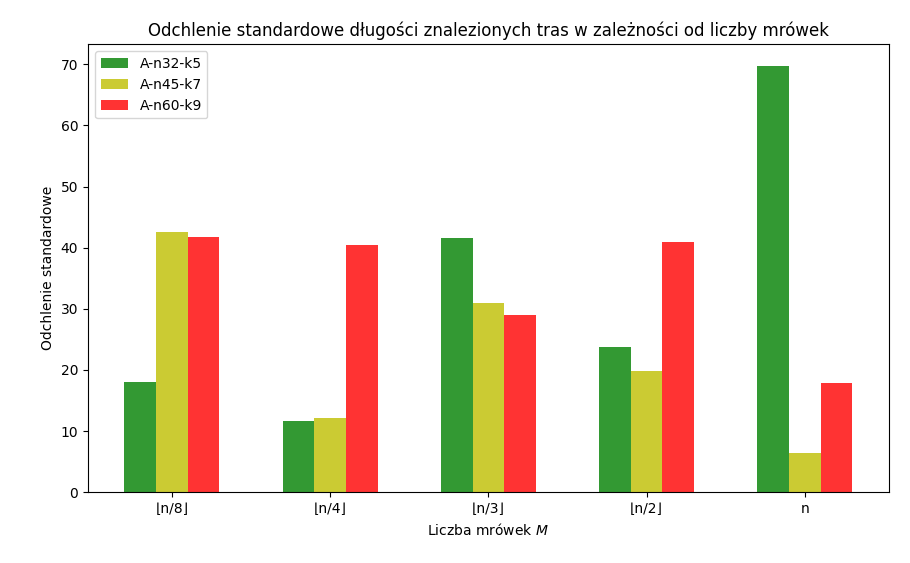
\includegraphics[width=0.75\textwidth]{deviation.png}
    \caption{Średnie odchylenie standardowe długości znalezionych tras w zależności od liczby mrówek}
    \label{fig:deviation}
\end{figure}

Na podstawie powyższych wykresów można dojść do wniosku, iż wraz ze wzrostem liczby mrówek, maleje średni błąd znalezionego rozwiązania. Zaskakujące jednak jest, iż ciężko znaleźć podobny trend jeśli chodzi o odchylenie standardowe. W tym przypadku nawet jeżeli wyniki dla wartości $N \in \left\{ \left\lfloor\frac{n}{4}\right\rfloor, \left\lfloor\frac{n}{2}\right\rfloor, n \right\}$ zdają się być równomiernie rozłożone w dwóch przypadkach testowych, przypadek trzeci podważa możliwość wyciągnięcia jednoznacznych wniosków.

Z tego powodu, w celu ostatecznego wyboru liczby mrówek dla następnych przypadków, wzięto pod uwagę również testy zbieżności.

Aby określić optymalny próg iteracji potrzebny do osiągnięcia zbieżności, przeanalizowane zostały długości tras znalezionych w kolejnych iteracjach. Po ustaleniu maksymalnej liczby iteracji na $1000$, okazało się iż w znacznej części testów wartość bliska oczekiwanej była znaleziona niemalże na samym początku. Mimo tego, stopniową poprawę wyników można było zaobserwować w niektórych testach aż do $1000$ iteracji. Jednak we wszystkich przypadkach, po dwusetnej iteracji poprawa wyników była niewielka, w szczególności biorąc pod uwagę konieczność kilkukrotnie dłuższego działania programu. Dokładniejsze przedstawienie tych wyników dla trzech przypadków testowych przedstawiają rysunki \ref{fig:iterations32}, \ref{fig:iterations45}, \ref{fig:iterations60}.

\begin{figure}[H]
    \centering
    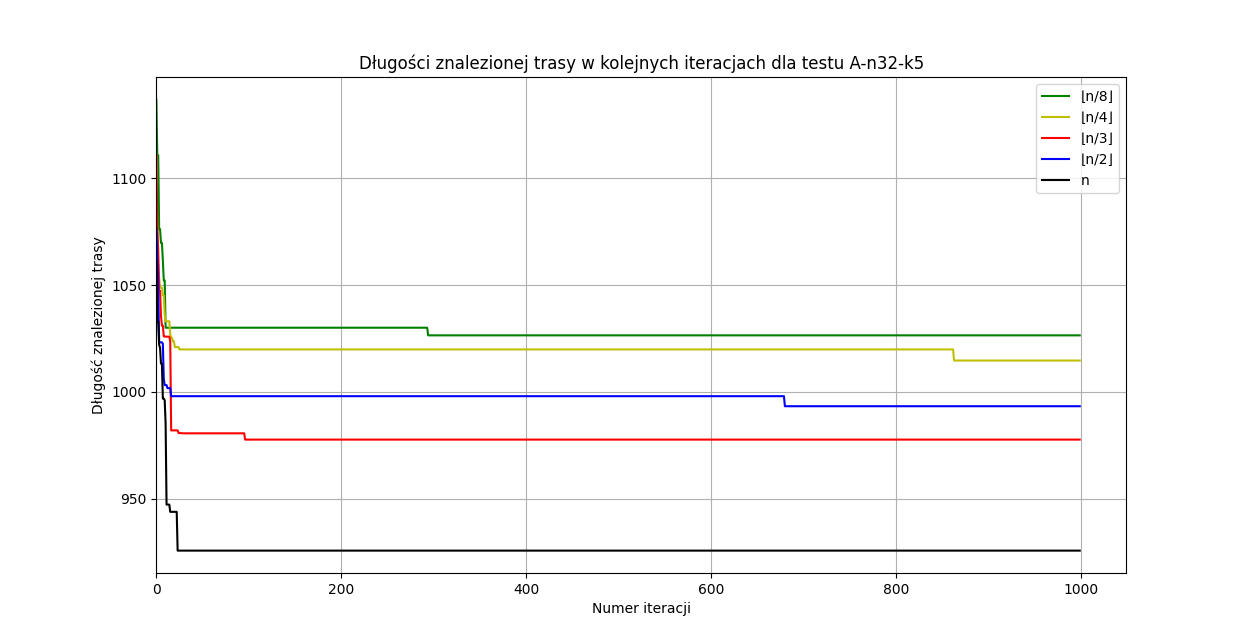
\includegraphics[width=0.75\textwidth]{iterations_32.png}
    \caption{Analiza zbieżności dla danych z pliku \textit{A-n32-k5}}
    \label{fig:iterations32}
\end{figure}

\begin{figure}[H]
    \centering
    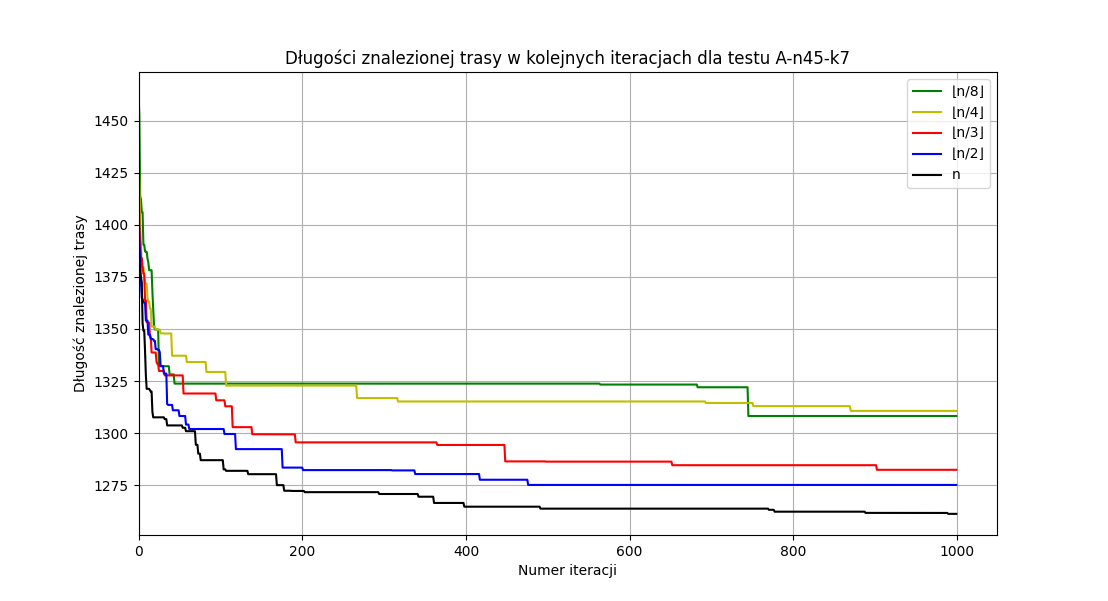
\includegraphics[width=0.75\textwidth]{iterations_45.png}
    \caption{Analiza zbieżności dla danych z pliku \textit{A-n45-k7}}
    \label{fig:iterations45}
\end{figure}

\begin{figure}[H]
    \centering
    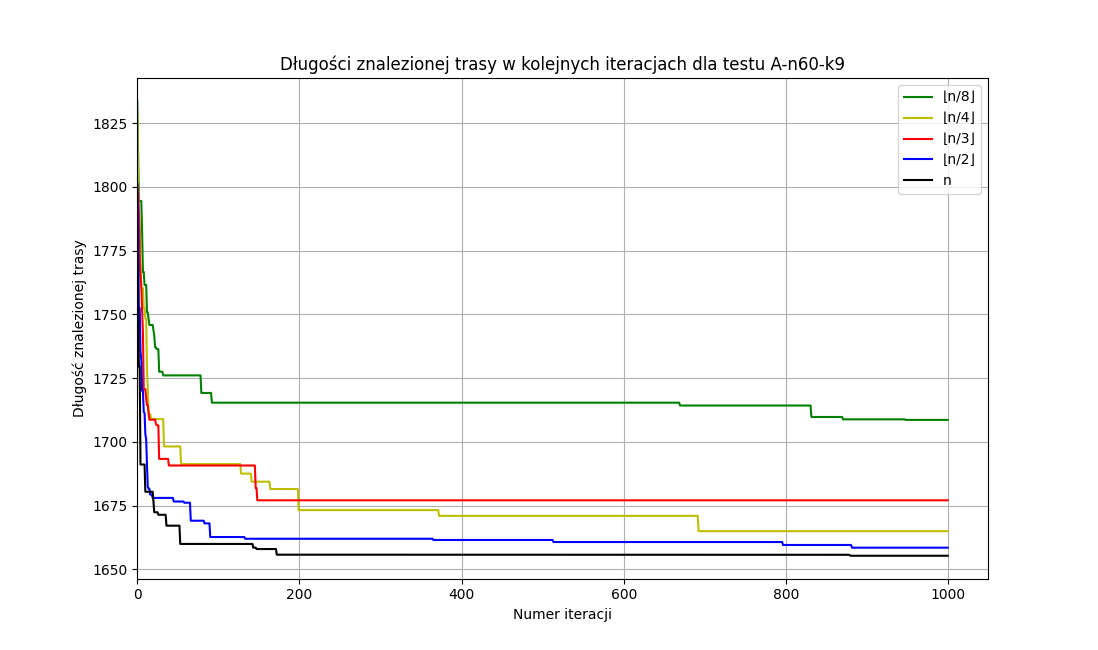
\includegraphics[width=0.75\textwidth]{iterations_60.png}
    \caption{Analiza zbieżności dla danych z pliku \textit{A-n60-k9}}
    \label{fig:iterations60}
\end{figure}

Warto zauważyć, że wraz ze wzrostem liczby mrówek, rosła również szybkość uzyskania zbieżności, w ten sposób uzasadniając wybór większej liczby mrówek do dalszej analizy. Przyjętymi wartościami parametrów były więc:
\begin{itemize}
    \item $N = n$
    \item $M = 200$  
\end{itemize}

\subsection{Wybór parametrów $\alpha$ i $\beta$}
Kolejnym etapem testów, było wybranie wartości parametrów $\alpha$ oraz $\beta$ określających skłonność mrówek do wybierania ścieżek heurystycznie bądź kierując się feromonami. Parametry te brane są pod uwagę przy wyznaczaniu wagi z jaką dani odbiorcy rozważani będą przy wyborze kolejnego miejsca docelowego, zgodnie ze wzorem:
\begin{equation*}
    w_{ij}^{(k)}(t) = \left[ \tau_{ij}(t) \right]^\alpha \left[ \frac{1}{d_{ij}}\right]^\beta
,\end{equation*} gdzie:
\begin{itemize}
    \item $w_{ij}^{(k)}(t)$ - waga wyboru przez mrówkę $t$ drogi od obecnego odbiorcy $i$ do odbiorcy $j$ w iteracji $k$
    \item $\tau_{ij}(t)$ - ilość feromonów na drodze od $i$ do $j$ w iteracji $t$
    \item $d_{ij}$ - dystans pomiędzy odbiorcami $i$ oraz $j$
\end{itemize}

Wybór spośród wszystkich możliwych $j$ jest następnie dokonywany w sposób pseudolosowy, biorąc pod uwagę właśnie wyznaczoną w ten sposób wagę. 

Przyjmując jako punkt wyjścia wartości $\alpha = 1$ i $\beta = 5$, przetestowane zostały różne kombinacje wartości z ich otoczenia: $\alpha \in \left\{ 0.5, 1, 1.5, 2, 3 \right\}$ oraz $\alpha \in \left\{ 3, 4, 4.5, 5, 5.5, 6, 7 \right\}$. Dla każdej możliwej kombinacji, przeprowadzono testy dla 5 wartości ziarna generatora liczb pseudolosowych oraz 3 zbiorów testowych.

Tendencje zmian błędu względnego pomiędzy rozwiązaniem znalezionym a rozwiązaniem optymalnym przedstawia rysunek \ref{fig:alphabeta}.

\begin{figure}[H]
    \centering
    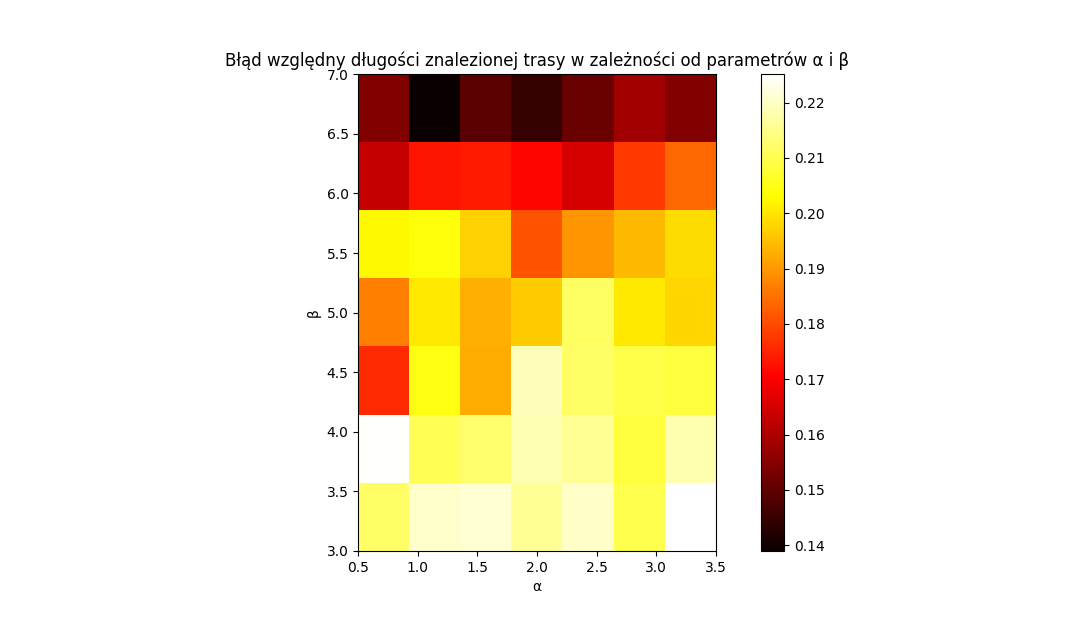
\includegraphics[width=0.85\textwidth]{alphabeta.png}
    \caption{Średni błąd względny długości znalezionych tras w zależności od wartości $\alpha$ oraz $\beta$}
    \label{fig:alphabeta}
\end{figure}

Ciekawym wnioskiem z przeprowadzonego eksperymentu jest fakt, iż dla wybranych danych testowych wartość błędu maleje wraz ze wzrostem wartości parametru $\beta$. Z kolei wartość $\alpha$ nie ma aż tak dużego wpływu. Na podstawie wyników tego etapu eksperymentów, do dalszej analizy przyjęto:
\begin{itemize}
    \item $\alpha = 1$
    \item $\beta = 7$  
\end{itemize}

\subsection{Wybór współczynnika parowania feromonów $\rho$}
Parametr $\rho \in \left(0, 1\right)$ decyduje o szybkości parowania feromonów zarówno ze ścieżek odwiedzanych, jak i nieodwiedzanych, definiując wartość feromonu po procesie parowania jako:
$$\tau_{ij}^{(k+1)} = (1-\rho)\tau_{ij}^{(k)} ,$$ gdzie $\tau_{ij}^{(k)}$ oznacza ilość feromonu na drodze między odbiorcami $i$ oraz $j$ na początku iteracji o numerze $k$.

Łatwo zauważyć, że większa wartość parametru $\rho$ wpłynie na szybsze parowanie feromonu. Wartości błędów wyniku dla testów przeprowadzonych dla $\rho \in \left\{ 0.3, 0.4, 0.5, 0.6, 0.7 \right\}$ przedstawione zostały na rysunku \ref{fig:rho}.

\begin{figure}[H]
    \centering
    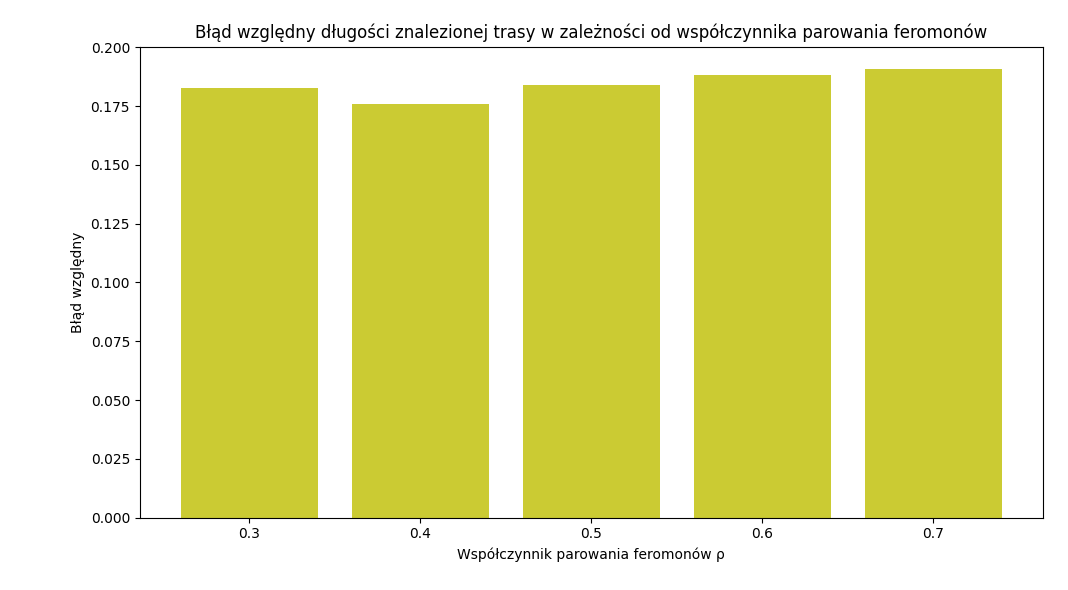
\includegraphics[width=0.75\textwidth]{rho.png}
    \caption{Średni błąd względny długości znalezionych tras w zależności od wartości $\rho$}
    \label{fig:rho}
\end{figure}

W wyniku testów okazało się, iż wpływ współczynnika $\rho$ na wartość błędu dla przyjętego zbioru testowego jest znikomy. Ostatecznie do dalszych testów przyjęta została wartość dla której osiągnięto nieznacznie lepsze wyniki, a więc:
\begin{itemize}
    \item $\rho = 0.4$
\end{itemize}

\subsection{Wybór parametru uaktualniania ścieżki feromonowej $Q$}
Współczynnik $Q$, początkowo wprowadzony jako $1$, definiuje ilość feromonów odkładanych przez mrówki na znalezionych ścieżkach jako:
\begin{equation*}
    \Delta\tau_{ij}^{(k)}(t) =
    \begin{cases}
      \frac{Q}{len\left(T^{(k)}(t)\right)} & \text{jeśli $ij \in T^{(k)}(t)$}\\
      0 & \text{w przeciwnym przypadku}
    \end{cases},
\end{equation*}
gdzie $T^{(k)}(t)$ oznacza całą trasę mrówki o indeksie $t$ w iteracji $k$, $len\left(T^{(k)}(t)\right)$ jej długość, a $\Delta\tau_{ij}^{(k)}(t)$ - ilość feromonów dołożoną przez mrówkę $t$ w iteracji $k$ pomiędzy odbiorcami $i$ oraz $j$.

Także w tym przypadku zdecydowano się na analizę średniej wartości błędu względnego w kolejnych testach, przedstawiając wyniki na rysunku \ref{fig:q}

\begin{figure}[H]
    \centering
    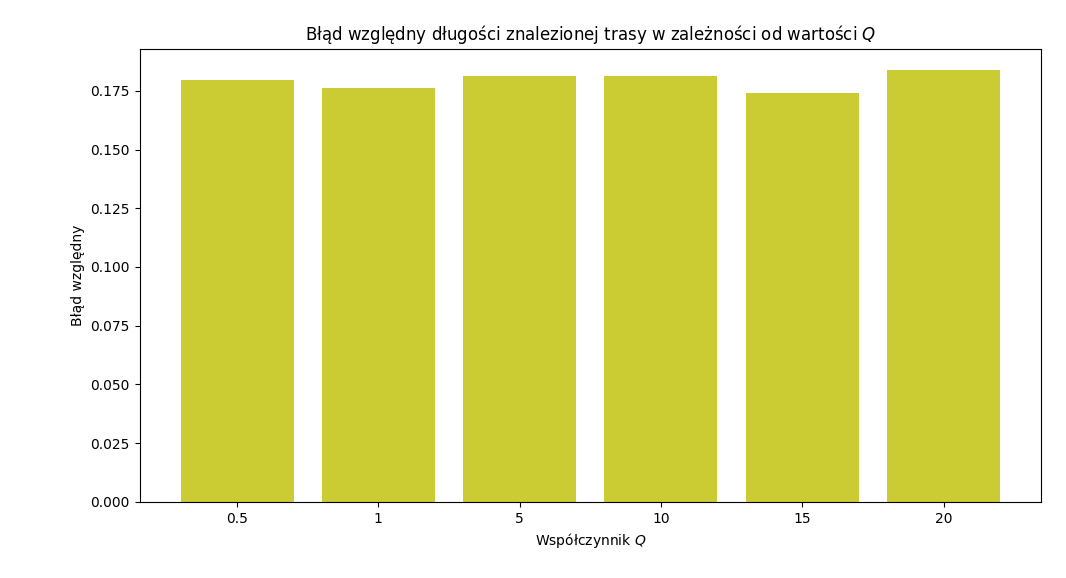
\includegraphics[width=0.75\textwidth]{q.png}
    \caption{Średni błąd względny długości znalezionych tras w zależności od wartości $Q$}
    \label{fig:q}
\end{figure}

W przypadku parametru $Q$, wyniki eksperymentów pozornie przypominają wyniki dla wartości $\rho$ - błąd zależy w niewielkim stopniu od wybranej wartości współczynnika. Jednak w tym przypadku nie istniał żaden sensowny trend utrzymujący się dla kilku zbiorów testowych, a nawet dla tego samego zbioru przy różnych wartościach ziarna generatora. Dla tych samych danych wejściowych, wyniki przy zastosowaniu różnych ziaren generatora liczb pseudolosowych potrafiły znaleźć się nawet po przeciwnych stronach spektrum - dla jednego ziarna wynik przy pewnej wartości $Q_0$ był najlepszy, dla innego ziarna z kolei - najgorszy, różniąc się przy tym o kilkanaście procent. Z tego powodu porównano dodatkowo średnie odchylenie standardowe wyników, prezentując rezultaty na rysunku \ref{fig:deviationq}.

\begin{figure}[H]
    \centering
    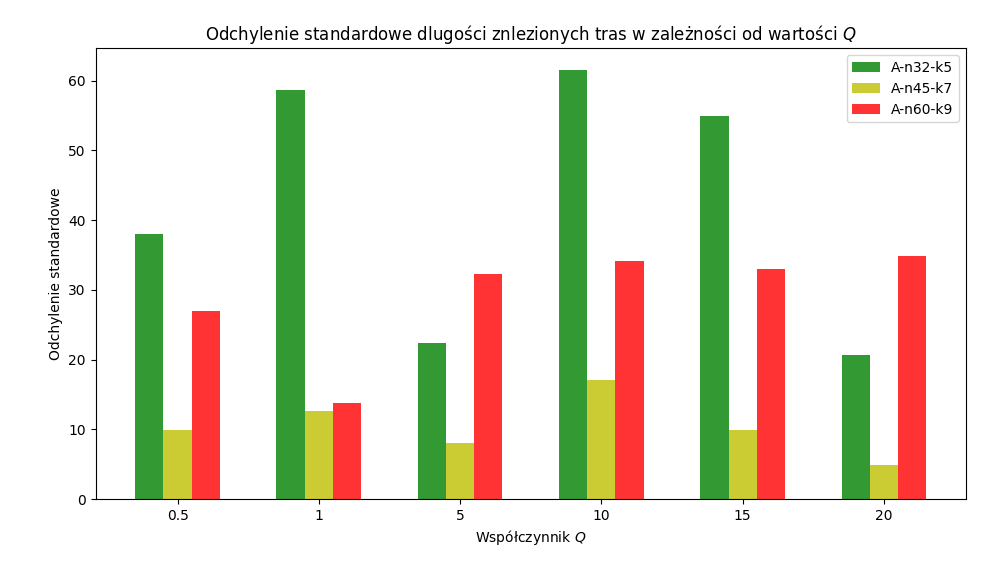
\includegraphics[width=0.75\textwidth]{deviation_q.png}
    \caption{Średnie odchylenie standardowe długości znalezionych tras w zależności od wartości $Q$}
    \label{fig:deviationq}
\end{figure}

Na podstawie obu powyższych zestawień, do dalszych testów subiektywnie wybrano wartość przedstawiającą najbardziej stabilne wyniki dla większości testów wyniki, czyli
\begin{itemize}
    \item $Q = 20$
\end{itemize}

\section{Hipotezy badawcze}
Głównym celem projektu było zbadanie czterech hipotez dotyczących wzajemnego porównania wszystkich czterech zaimplementowanych algorytmów rozwiązujących CVRP. W wyniku przeprowadzonych eksperymentów udało się całkowicie potwierdzić jedną z nich, kolejne dwie znalazły częściowe potwierdzenie, zaś jedna okazała się błędna. Więcej informacji o postawionych hipotezach i ich weryfikacji przedstawiono w kolejnych podsekcjach.

\subsection{Wyniki działania algorytmu z wyborem mrówek elitarnych będą w dużym stopniu zależne od wybrania liczby mrówek elitarnych, a optymalna wartość tej liczby będzie się różnić dla różnych testów}
Wynik: Hipoteza \textbf{częściowo potwierdzona}.

Podobnie do parametrów sprawdzanych w poprzedniej sekcji \textit{\ref{sec:experiments} \nameref{sec:experiments}}, również w tym przypadku publikacje~\cite{Dorigo1996} \cite{Dorigo1999} sugerują optymalną wartość parametru. W tym przypadku sugerowana wartość to $8$. Jednak aby dokładniej przeanalizować zachowanie algorytmu w zależności od właśnie tego parametru, przetestowano wartości ze zbioru $e \in \left\{ 6, 7, 8, 9, 10 \right\}$. Na rysunkach \ref{fig:errors_e} i \ref{fig:deviation_e} przedstawiono odpowiednio zależność średniego błędu względnego wyniku oraz średniego odchylenia standardowego w zależności od wspomnianych wartości parametru. 

\begin{figure}[H]
    \centering
    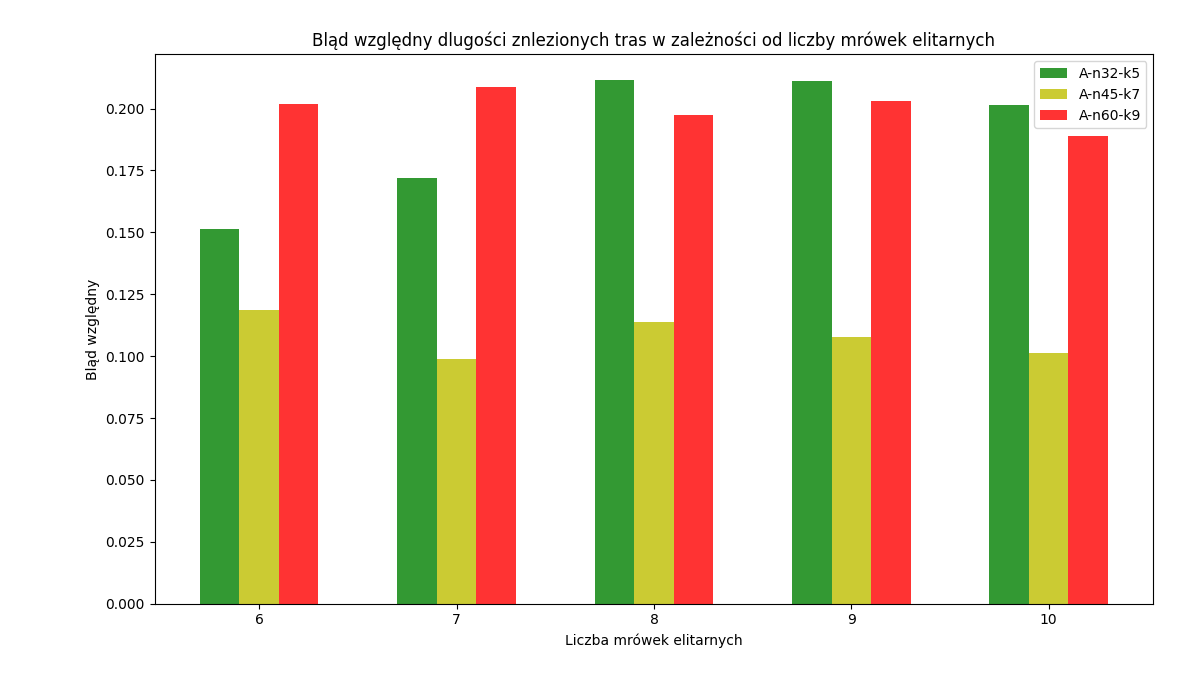
\includegraphics[width=0.75\textwidth]{errors_e.png}
    \caption{Średni błąd względny długości znalezionych tras w zależności od liczby mrówek elitarnych}
    \label{fig:errors_e}
\end{figure}

\begin{figure}[H]
    \centering
    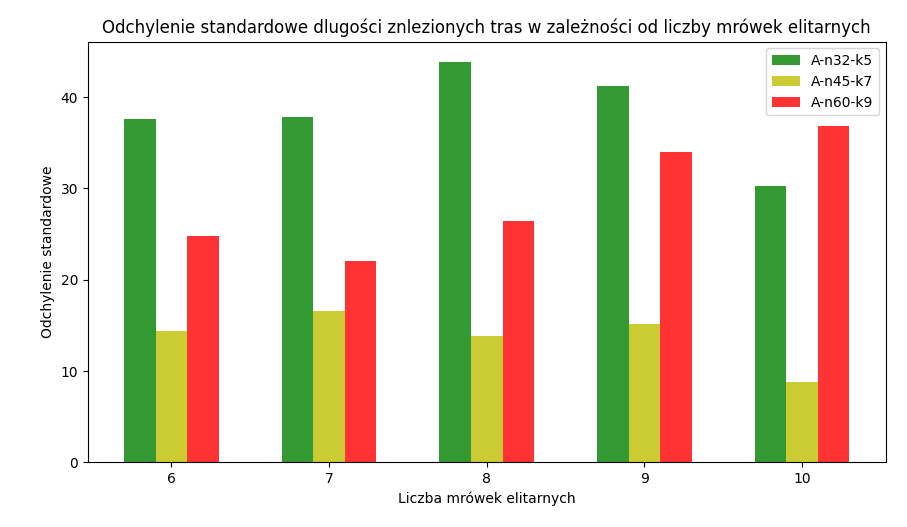
\includegraphics[width=0.75\textwidth]{deviation_e.png}
    \caption{Średnie odchylenie standardowe długości znalezionych tras w zależności od liczby mrówek elitarnych}
    \label{fig:deviation_e}
\end{figure}

Analizując przedstawione na wykresach wyniki eksperymentów, hipoteza uznana została za częściowo potwierdzoną. Wartość liczby mrówek elitarnych wpływa na jakość rozwiązania, jednak w znacznie mniejszym stopniu niż było to podejrzewane.

Kolejnym spostrzeżeniem z przeprowadzonej analizy jest wzajemna zależność optymalnej liczby mrówek elitarnych od wielkości zbioru testowego. Dla $32$ miast, najlepszy wynik dało $6$ mrówek, dla $45$ było to $7$, zaś dla $60$ wartość optymalna wynosiła $10$. Na podstawie tej obserwacji słuszne zdaje się być uzależnienie liczby mrówek elitarnych właśnie od liczby miast, zamiast przyjmować stałą wartość dla wszystkich testów. Z tego też powodu, jako wartość reprezentatywną dla algorytmu przyjęte zostało $e = \left\lfloor\frac{n}{6}\right\rfloor$.

\subsection{Algorytm z wyborem mrówek elitarnych zbiegnie szybciej niż algorytm podstawowy, jednak znajdzie gorsze rozwiązanie}
Wynik: Hipoteza \textbf{odrzucona}

W przypadku tego testu, tak jak i wszystkich kolejnych, rozszerzono zbiór testów do 5 zestawów danych: \mbox{\textit{A-n32-k5}}, \textit{A-n39-k5}, \textit{A-n45-k7}, \textit{A-n53-k7}, \textit{A-n60-k9}. Następnie, dla każdego zestawu, przeprowadzone zostały testy dla 5 różnych wartości ziarna generatora liczb pseudolosowych, opisanych w \textit{\ref{sec:experiments} \nameref{sec:experiments}}.
Dla każdego zbioru testowego analizie poddane były: czas działania algorytmu, wartości znalezionego rozwiązania w kolejnych iteracjach, błąd względny znalezionego rozwiązania oraz odchylenie standardowe tego rozwiązania. Wyniki eksperymentów przedstawiają odpowiednio rysunki \ref{fig:iterations_elitist}, \ref{fig:time_elitist}, \ref{fig:errors_elitist} oraz \ref{fig:deviation_elitist}.

Istotną informacją jest również zmiana sposobu liczenia odchylenia standardowego: od tej pory analizowana odległość od wartości średniej została dodatkowo podzielona przez tę wartość, umożliwiając względne porównanie wyników dla różnych zbiorów testowych.  

Pierwszą z części hipotezy było sprawdzenie czy wprowadzenie mrówek elitarnych spowoduje szybsze zbiegnięcie wyniku do jakiejś wartości, która następnie nie będzie się zmieniała w kolejnych iteracjach. Mimo, iż wydawało się to intuicyjnie poprawne, testy wskazały inne wyniki. Algorytm bez ulepszenia w większości przypadków szybciej osiągał niemal stabilny poziom, po którym następowały wyłącznie nieznaczne zmiany wartości. W przypadku ulepszenia z mrówkami elitarnymi, uzyskanie stałej wartości wymagało więcej iteracji bądź następujące zmiany były wyraźniejsze. Rysunek \ref{fig:iterations_elitist} przedstawia dokładniejsze zestawienie z podziałem na wykorzystane zbiory testowe.

Kolejnym aspektem poddanym analizie był czas działania obu algorytmów, który okazał się on być praktycznie jednakowy. Potwierdza to intuicję - ulepszenie dodające mrówki elitarne dodało wyłącznie stałą liczbę operacji w każdej iteracji. Przy tak długim czasie obliczeń w pojedynczej iteracji, czas ich działania okazał się niemalże pomijalny.

\begin{figure}[H]
    \centering
    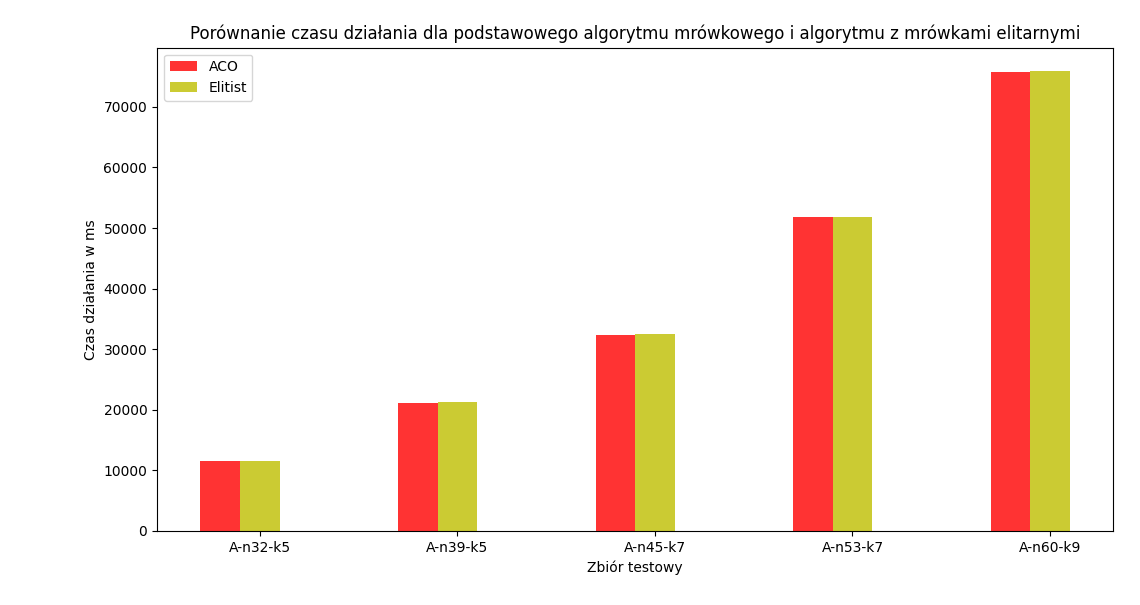
\includegraphics[width=0.75\textwidth]{time_elitist.png}
    \caption{Porównanie czasu działania dla podstawowego algorytmu mrówkowego i rozszerzenia z mrówkami elitarnymi}
    \label{fig:time_elitist}
\end{figure}

\begin{figure}[H]
     \centering
     \begin{subfigure}[b]{0.4\textwidth}
         \centering
         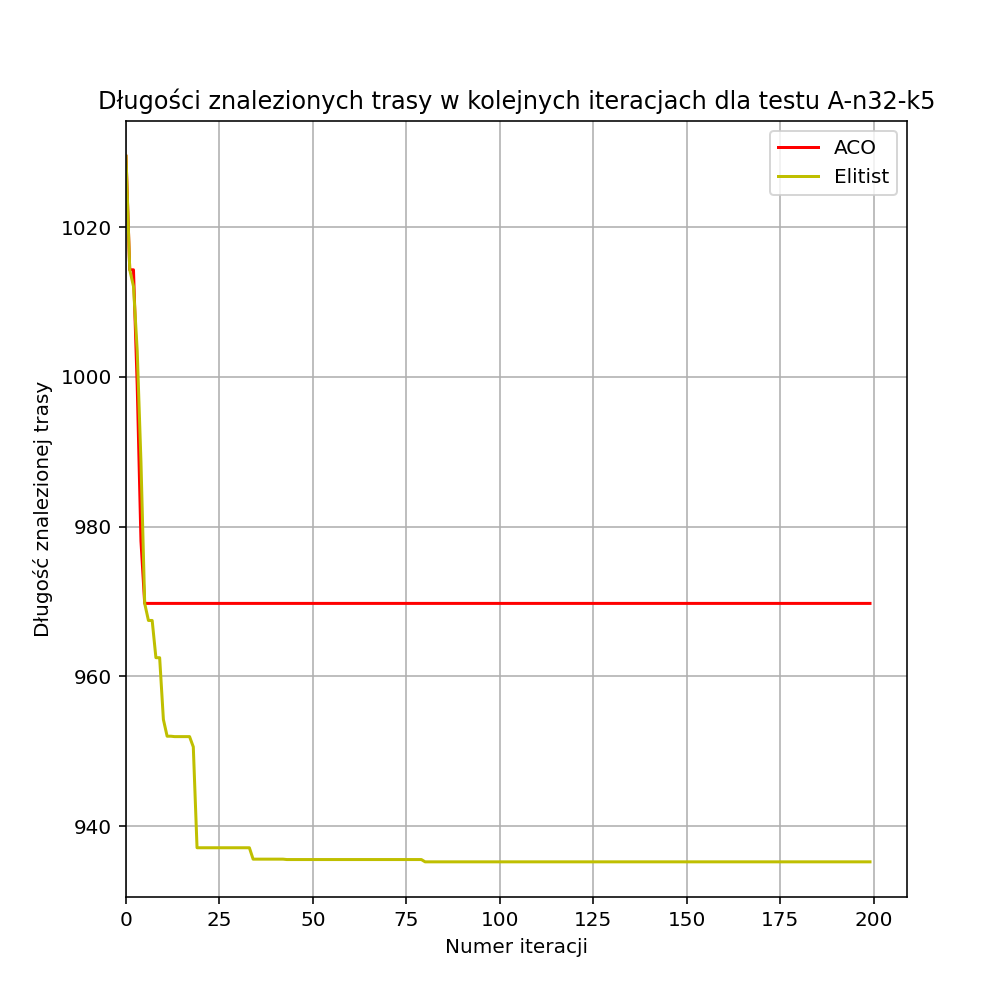
\includegraphics[width=\textwidth]{iterations_elitist_1.png}
         \caption{Test \textit{A-n32-k5}}
     \end{subfigure}
     \hfill
     \begin{subfigure}[b]{0.4\textwidth}
         \centering
         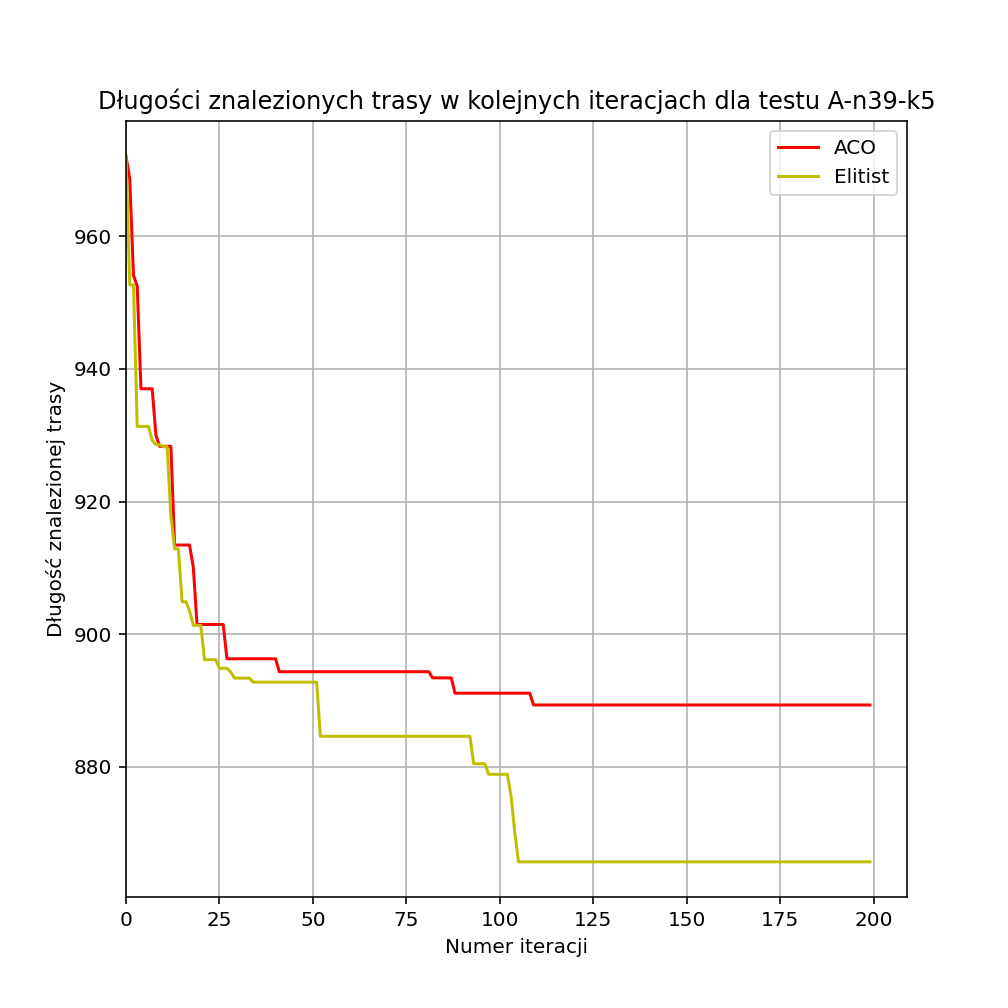
\includegraphics[width=\textwidth]{iterations_elitist_2.png}
         \caption{Test \textit{A-n39-k5}}
     \end{subfigure}
     \hfill
     \begin{subfigure}[b]{0.4\textwidth}
         \centering
         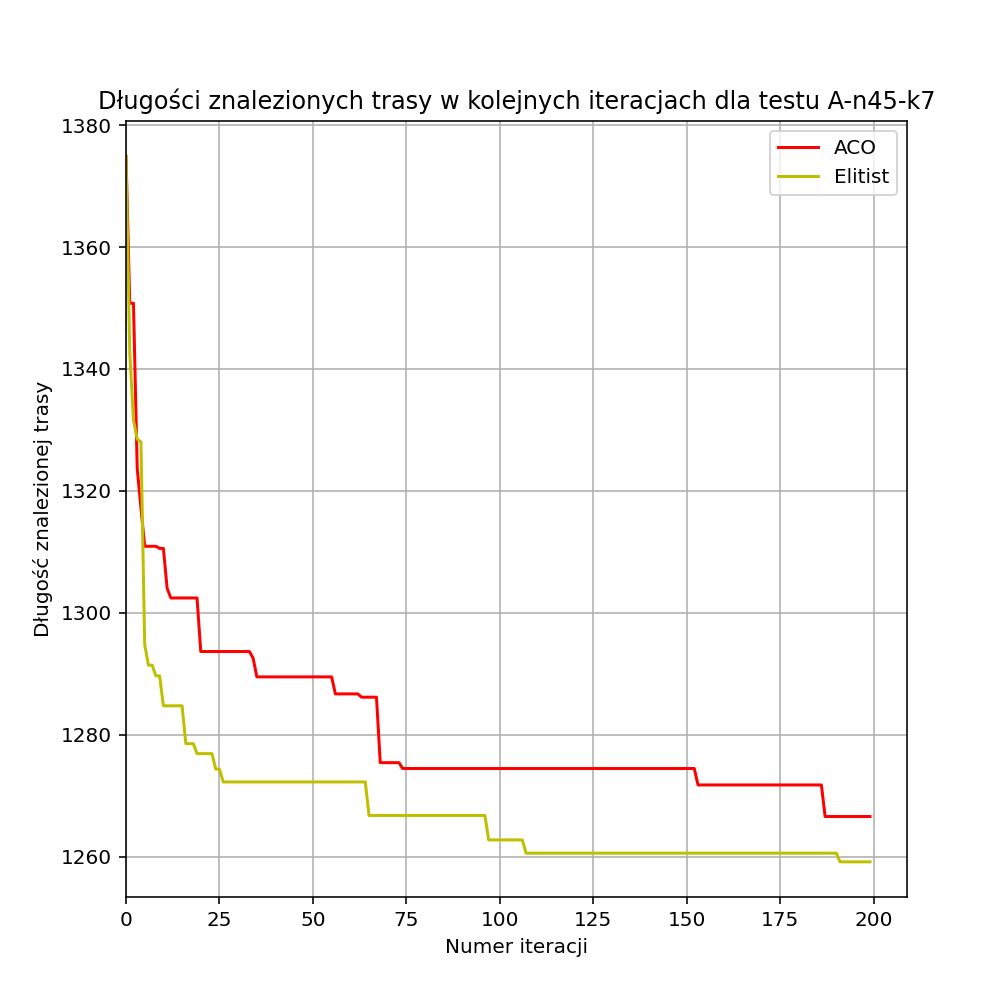
\includegraphics[width=\textwidth]{iterations_elitist_3.png}
         \caption{Test \textit{A-n45-k7}}
     \end{subfigure}
     \hfill
     \begin{subfigure}[b]{0.4\textwidth}
         \centering
         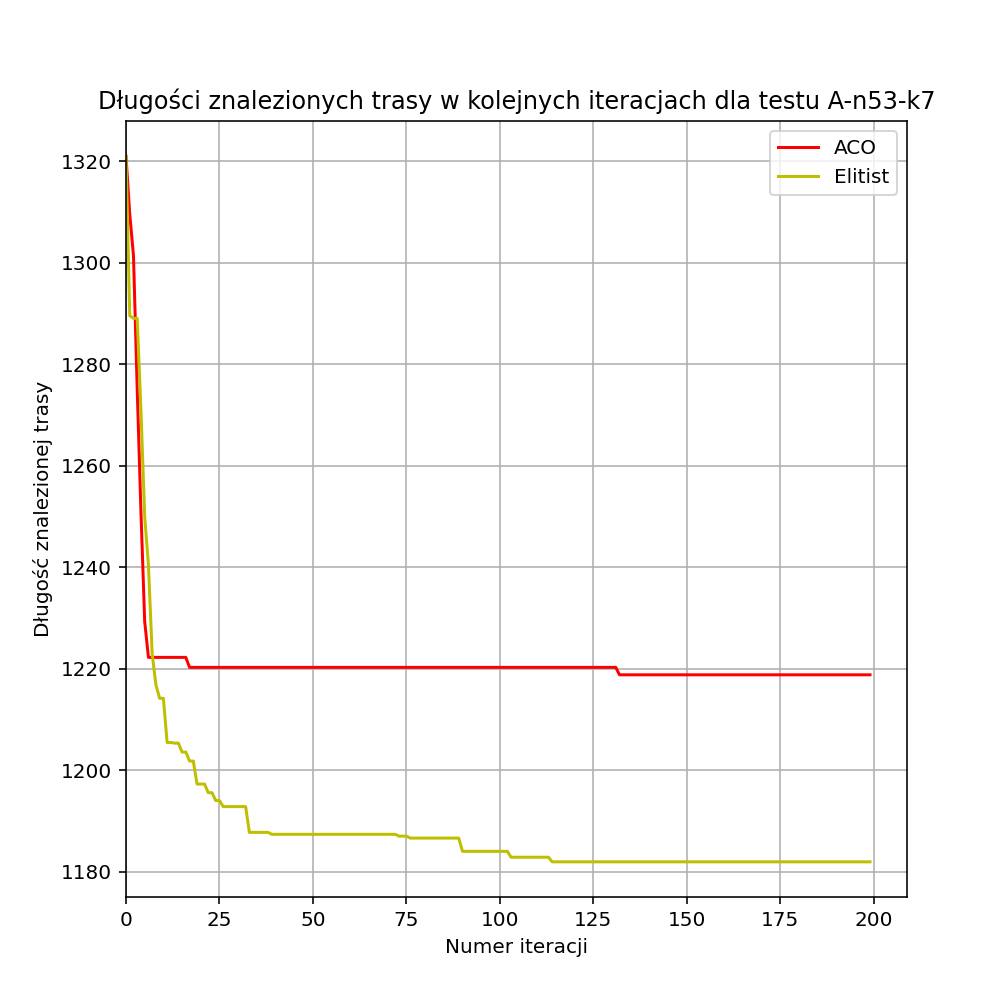
\includegraphics[width=\textwidth]{iterations_elitist_4.png}
         \caption{Test \textit{A-n53-k7}}
     \end{subfigure}
     \hfill
     \begin{subfigure}[b]{0.4\textwidth}
         \centering
         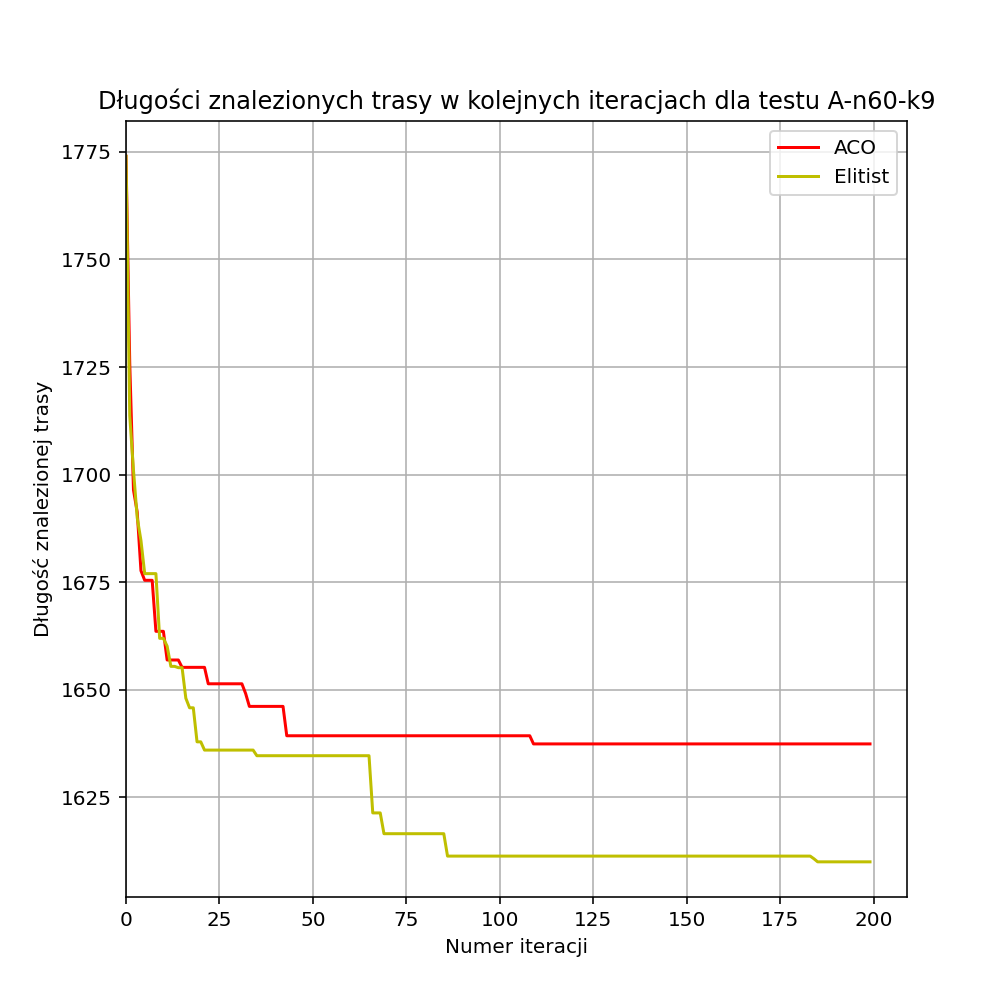
\includegraphics[width=\textwidth]{iterations_elitist_5.png}
         \caption{Test \textit{A-n60-k9}}
     \end{subfigure}
    \caption{Porównanie liczby iteracji dla podstawowego algorytmu mrówkowego i rozszerzenia z mrówkami elitarnymi}
    \label{fig:iterations_elitist}
\end{figure}

Następnym, a zarazem kluczowym aspektem testu było porównanie jakości podstawowej wersji algorytmu oraz wersji z dodanymi mrówkami elitarnymi. Wbrew hipotezie, dla każdego przypadku testowego, błąd wyniku znalezionego przez algorytm elitarny okazał się mniejszy niż dla podstawowej wersji algorytmu. Świadczy to oczywiście dobrze o zaimplementowanym ulepszeniu, gdyż pozwoliło ono poprawić wyniki podstawowej implementacji, działając w niemalże takim samym czasie.

\begin{figure}[H]
    \centering
    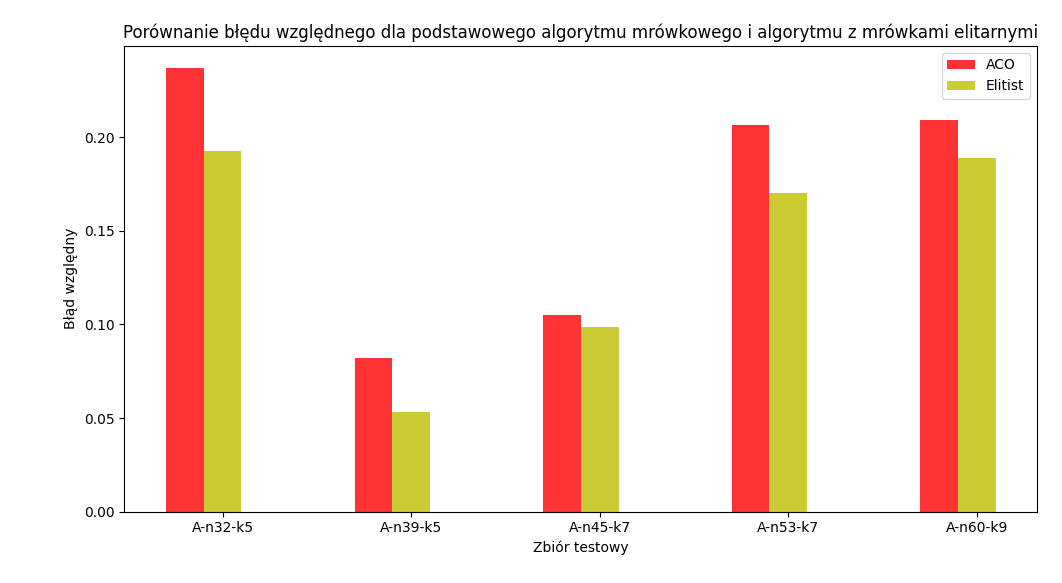
\includegraphics[width=0.75\textwidth]{errors_elitist.png}
    \caption{Porównanie błędu względnego dla podstawowego algorytmu mrówkowego i rozszerzenia z mrówkami elitarnymi}
    \label{fig:errors_elitist}
\end{figure}

O ile testy pozwoliły wysunąć jasne wnioski dotyczące ogólnej jakości rozwiązań, o tyle odchylenie standardowe wyników nie jest tak oczywiste do interpretacji. W tym przypadku brakuje jednakowego trendu w porównaniu obu metod. Dla dwóch mniejszych testów wyniki były bardziej stabilne w podstawowej wersji algorytmu, dla kolejnych dwóch - w ulepszonej, zaś dla największego testu obie implementacje dały podobne rezultaty. Wskazuje to interesujące pytanie do dalszych badań: czy algorytm z wyborem mrówek elitarnych będzie dawał mniej stabilne wyniki dla mniejszych zbiorów testowych?

\begin{figure}[H]
    \centering
    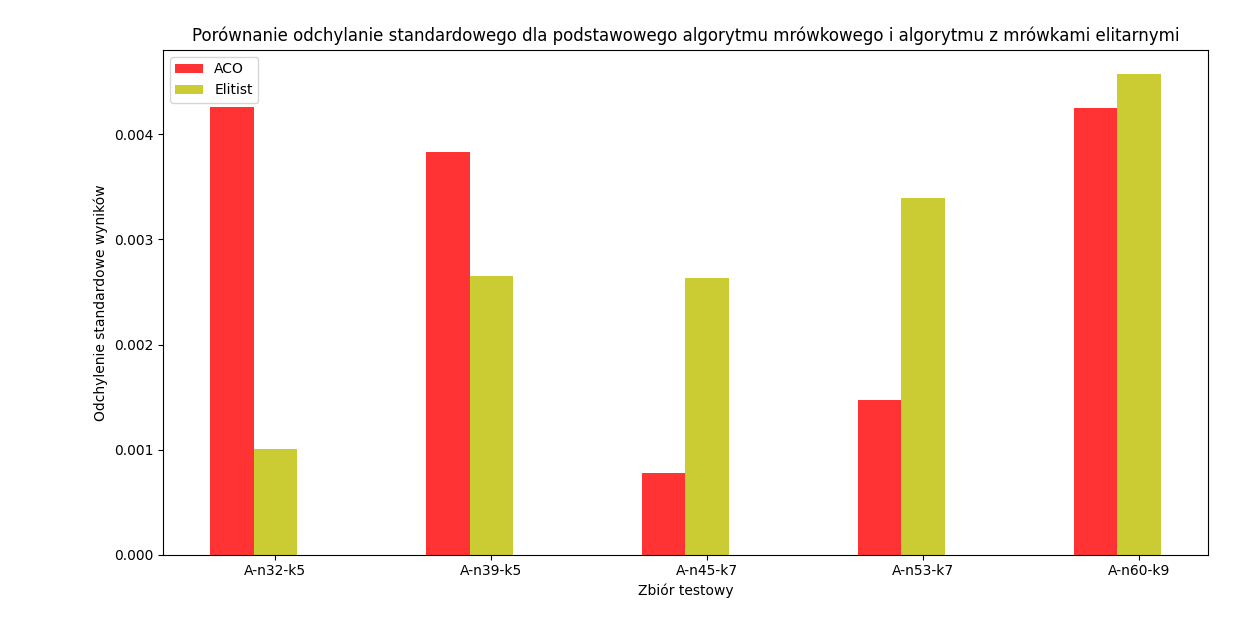
\includegraphics[width=0.75\textwidth]{deviation_elitist.png}
    \caption{Porównanie odchylenia standardowego dla podstawowego algorytmu mrówkowego i rozszerzenia z mrówkami elitarnymi}
    \label{fig:deviation_elitist}
\end{figure}

\subsection{Algorytm z odwróceniem częściowych ścieżek będzie wolniejszy niż algorytm podstawowy, jednak znajdzie bardziej optymalne rozwiązanie w mniejszej liczbie iteracji}
Wynik: Hipoteza \textbf{częściowo potwierdzona}

Podobnie jak przy porównaniu ulepszenia z mrówkami elitarnymi, w tym przypadku również testy opierały się na wywołaniu algorytmu ulepszonego oraz podstawowego dla kilku ziaren oraz kilku zbiorów testowych. Dla każdego zbioru testowego analizie poddane były: czas działania algorytmu, wartości znalezionego rozwiązania w kolejnych iteracjach, błąd względny znalezionego rozwiązania oraz odchylenie standardowe tego rozwiązania. Wyniki eksperymentów przedstawiają odpowiednio rysunki \ref{fig:time_enhanced}, \ref{fig:iterations_enhanced}, \ref{fig:errors_enhanced} oraz \ref{fig:deviation_enhanced}.

Najważniejszym etapem testów w przypadku porównania tych dwóch implementacji było zestawienie szybkości działania. Odwracanie wszystkich możliwych częściowych ścieżek (a konkretniej ich znajdowanie) jest operacją bardziej czasochłonną niż zwykła aktualizacja ilości feromonów. Z tego też powodu, istniało realne podejrzenie, że ulepszenie to okaże się dużo wolniejsze niż implementacja podstawowa. Wyniki przeprowadzonych testów potwierdziły te wątpliwości, jednak różnice w czasie działania były znacznie mniejsze niż początkowo przypuszczano.

\begin{figure}[H]
    \centering
    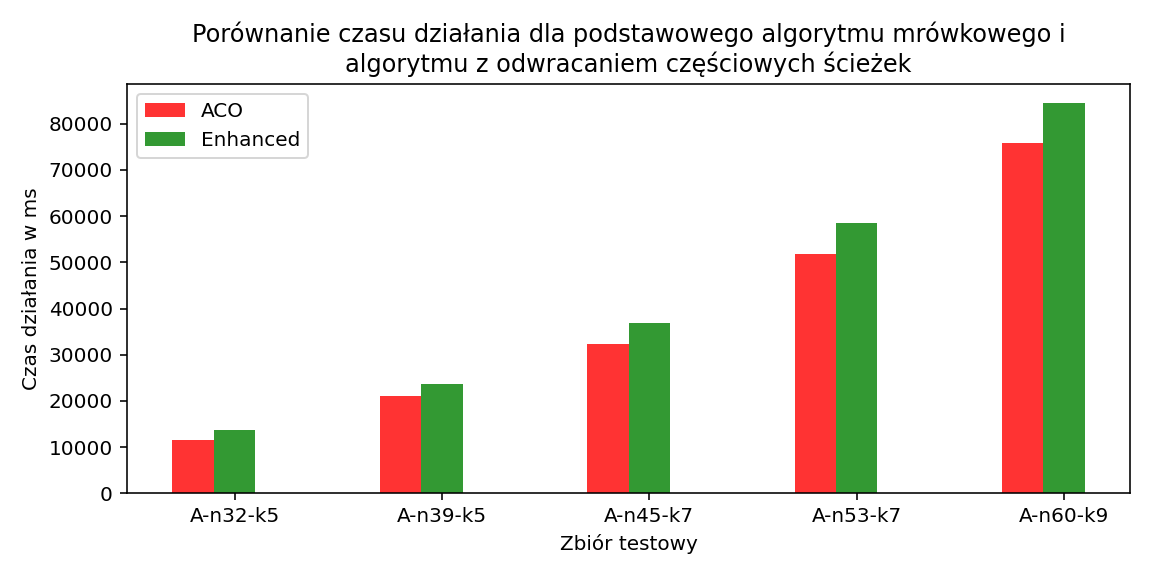
\includegraphics[width=0.75\textwidth]{time_enhanced.png}
    \caption{Porównanie czasu działania dla podstawowego algorytmu mrówkowego i rozszerzenia z odwracaniem częściowych ścieżek}
    \label{fig:time_enhanced}
\end{figure}

Jak widać z wykresów, odwracanie ścieżek spowodowało wzrost czasu działania programów dla każdego zbioru testowego, jednak różnice te mieściły się w granicach kilku/kilkunastu procent. Nie jest to co prawda wartość, którą można pominąć, jednak nie jest to również wzrost dyskwalifikujący analizowany algorytm z dalszych rozważań.

Kolejną częścią hipotezy była liczba iteracji potrzebna ulepszonej wersji algorytmu do znalezienia najlepszego rozwiązania. W tym przypadku, intuicyjnie rzecz biorąc, przeszukiwanie lokalnie podobnych rozwiązań miało potencjał doprowadzić metodę do szybszej zbieżności. Testy wykazały jednak odwrotny trend - algorytm poprawiał znalezione wyniki w iteracjach w których działanie podstawowej wersji było już ustabilizowane. Prawdopodobną przyczyną takiego stanu rzeczy był fakt, iż po znalezieniu rozwiązania bliższego optymalnemu, w każdej iteracji przeszukiwane były rozwiązania do niego podobne, wykazując w ten sposób chęć poprawy w każdej iteracji. Takiego zachowania oczywiście nie można spodziewać się po podstawowym algorytmie, który stara się w miarę możliwości ustabilizować przy lokalnie dobrym rozwiązaniu.

\begin{figure}[H]
     \centering
     \begin{subfigure}[b]{0.4\textwidth}
         \centering
         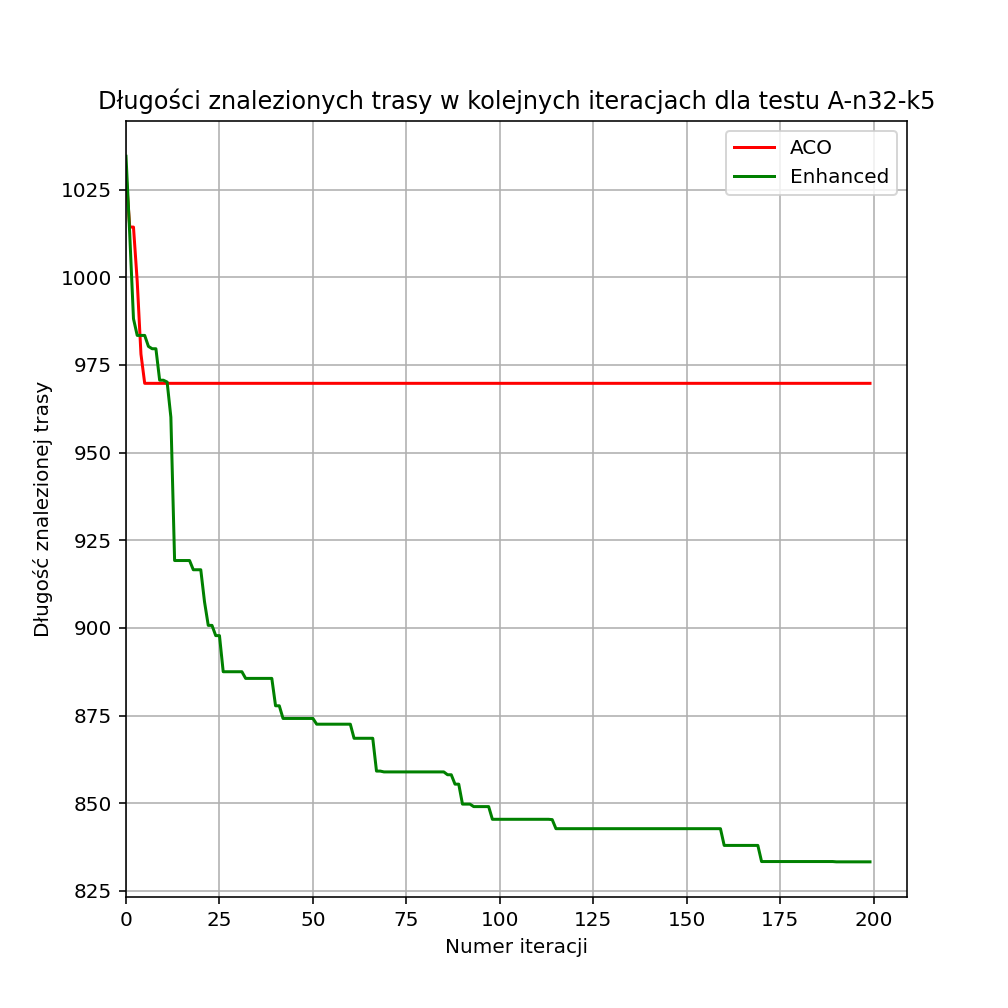
\includegraphics[width=\textwidth]{iterations_enhanced_1.png}
         \caption{Test \textit{A-n32-k5}}
     \end{subfigure}
     \hfill
     \begin{subfigure}[b]{0.4\textwidth}
         \centering
         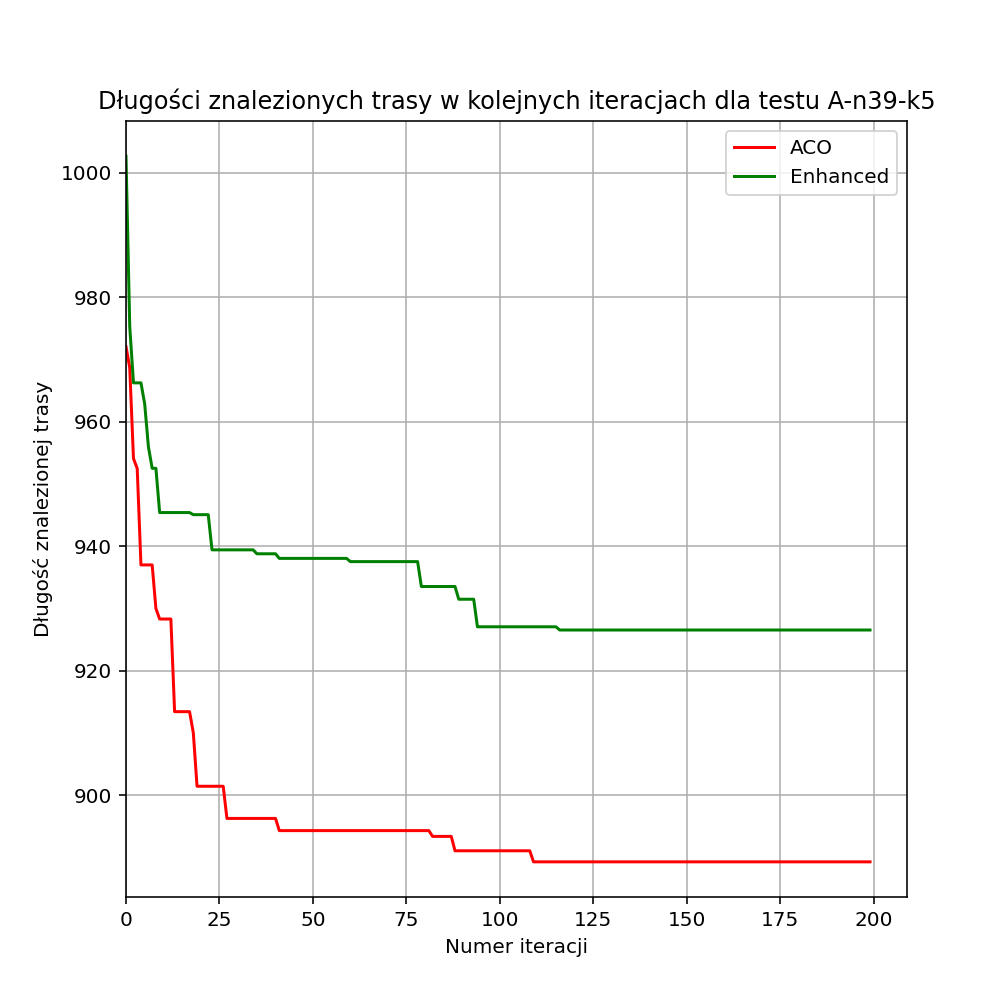
\includegraphics[width=\textwidth]{iterations_enhanced_2.png}
         \caption{Test \textit{A-n39-k5}}
     \end{subfigure}
     \hfill
     \begin{subfigure}[b]{0.4\textwidth}
         \centering
         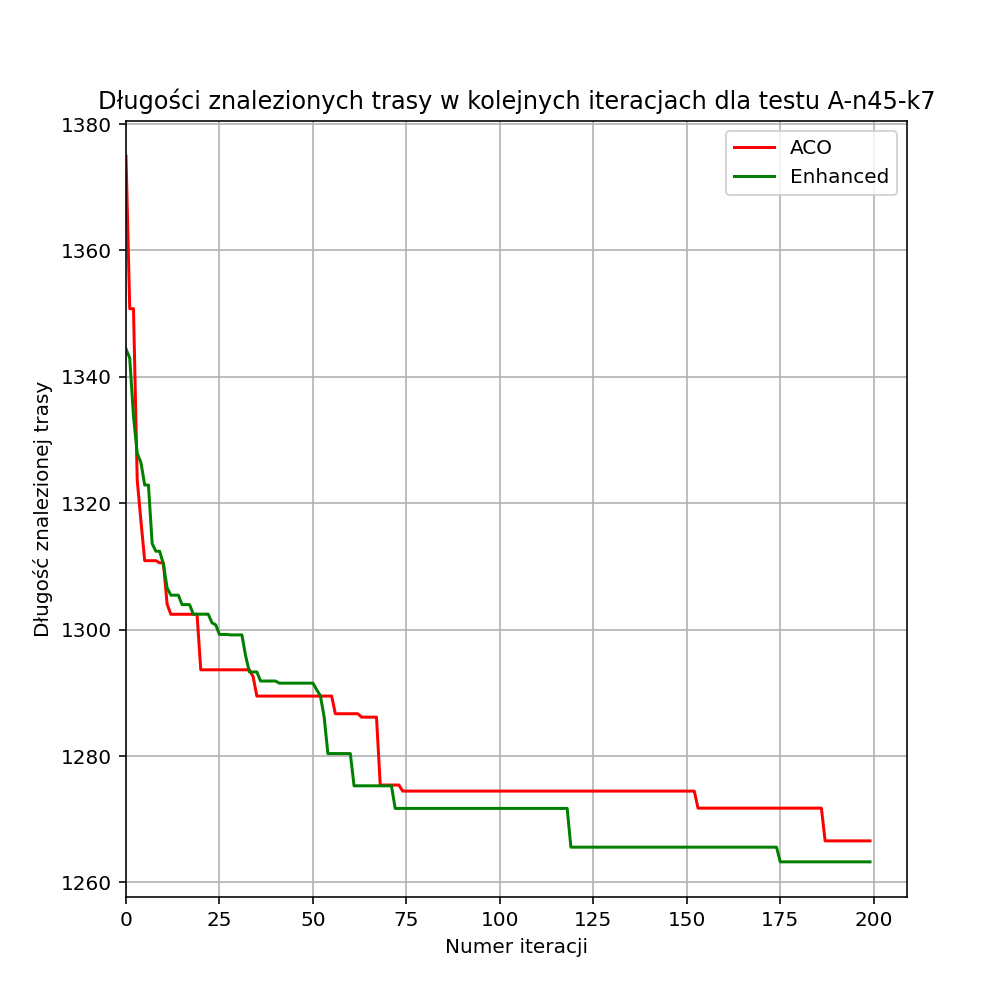
\includegraphics[width=\textwidth]{iterations_enhanced_3.png}
         \caption{Test \textit{A-n45-k7}}
     \end{subfigure}
     \hfill
     \begin{subfigure}[b]{0.4\textwidth}
         \centering
         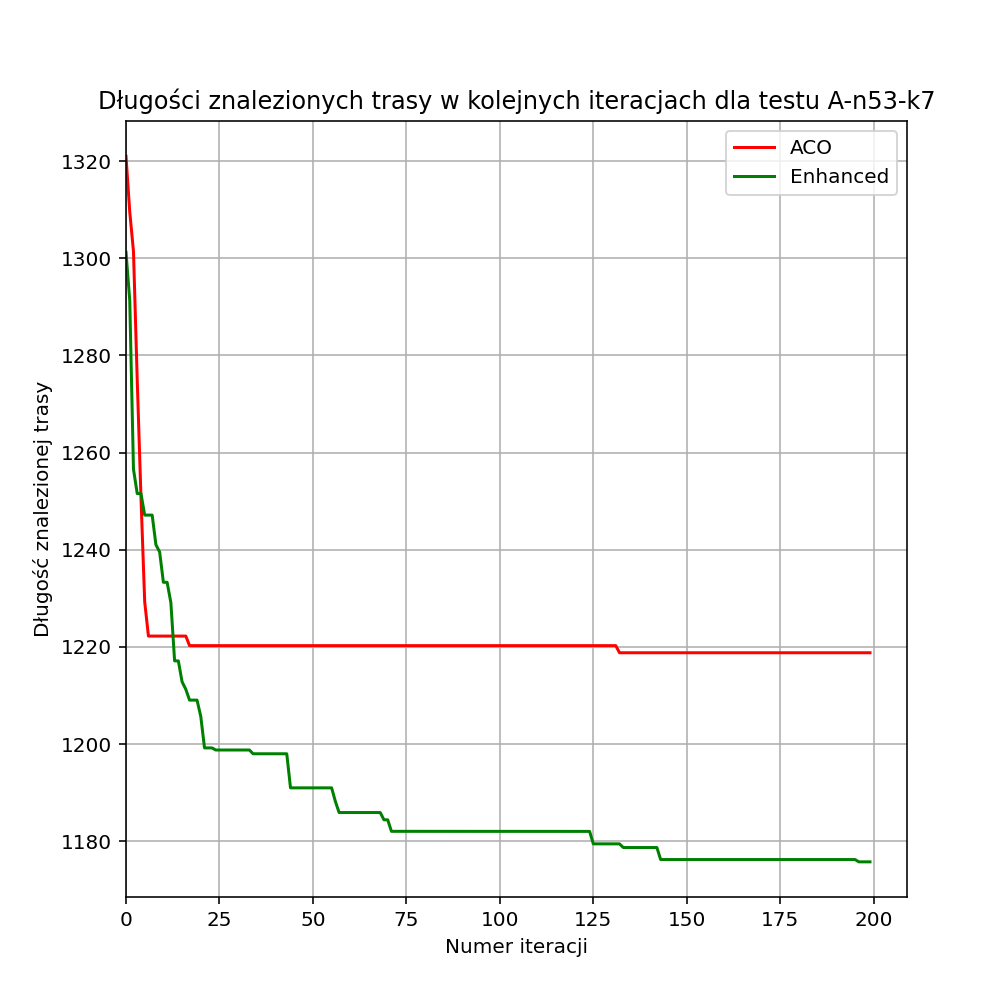
\includegraphics[width=\textwidth]{iterations_enhanced_4.png}
         \caption{Test \textit{A-n53-k7}}
     \end{subfigure}
     \hfill
     \begin{subfigure}[b]{0.4\textwidth}
         \centering
         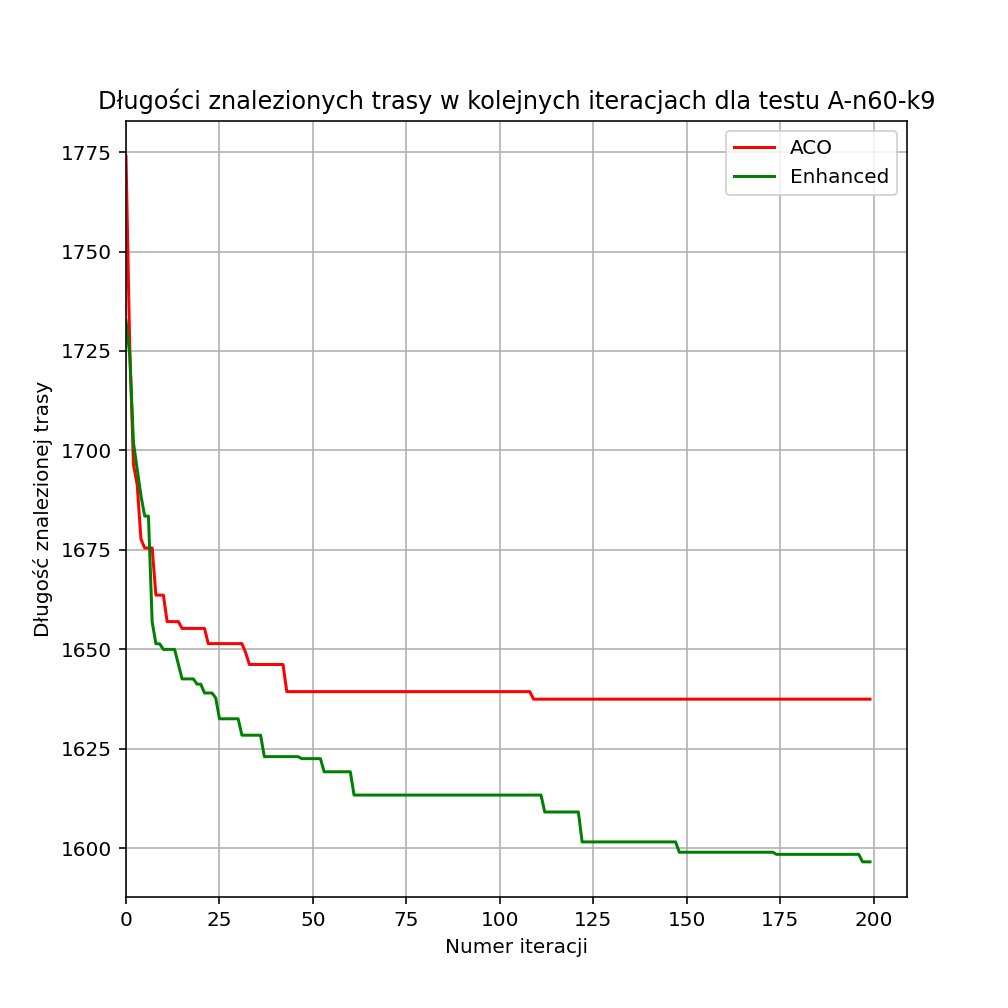
\includegraphics[width=\textwidth]{iterations_enhanced_5.png}
         \caption{Test \textit{A-n60-k9}}
     \end{subfigure}
    \caption{Porównanie liczby iteracji dla podstawowego algorytmu mrówkowego i rozszerzenia z odwracaniem częściowych ścieżek}
    \label{fig:iterations_enhanced}
\end{figure}

Przy stawianiu hipotez dotyczących tego ulepszenia, jego główną przewagą nad podstawową wersją algorytmu mrówkowego miało być znajdowanie lepszego rozwiązania, nawet kosztem dłuższego czasu działania. Jak widać po przeprowadzonych eksperymentach, okazało się to słusznym kierunkiem w większości przypadków testowych. Jednakże, dla jednego ze zbiorów, algorytm zwracał wyniki znacznie gorsze niż podstawowa implementacja. Jest to bardzo ciekawa anomalia, otwierająca potencjalny kierunek do dalszej analizy. Warto jednak zauważyć że przypadek ten opierał się na dużej liczbie miast oraz małej liczbie dostępnych samochodów. Może to sugerować, że działanie tego ulepszenia nie daje najlepszych rezultatów gdy analizie poddawane są długie fragmenty tras.

\begin{figure}[H]
    \centering
    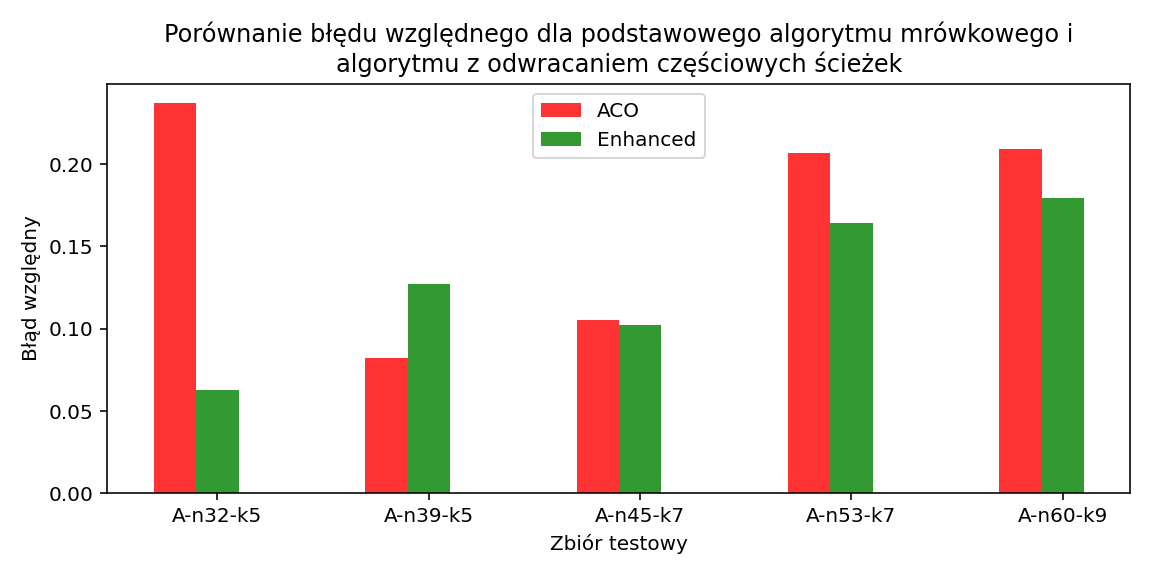
\includegraphics[width=0.75\textwidth]{errors_enhanced.png}
    \caption{Porównanie błędu względnego dla podstawowego algorytmu mrówkowego i rozszerzenia z odwracaniem częściowych ścieżek}
    \label{fig:errors_enhanced}
\end{figure}

Kolejną ciekawą cechą proponowanego ulepszenia okazało się być również odchylenie standardowe znalezionych rozwiązań. W odróżnieniu do poprzedniego ulepszenia, w tym przypadku wyniki zdają się być dużo bardziej zrównoważone. Dla trzech zbiorów testowych proponowane ulepszenie dawało wyniki bardziej stabilne niż podstawowa wersja algorytmu, w pozostałych dwóch tylko nieznacznie gorsze.

\begin{figure}[H]
    \centering
    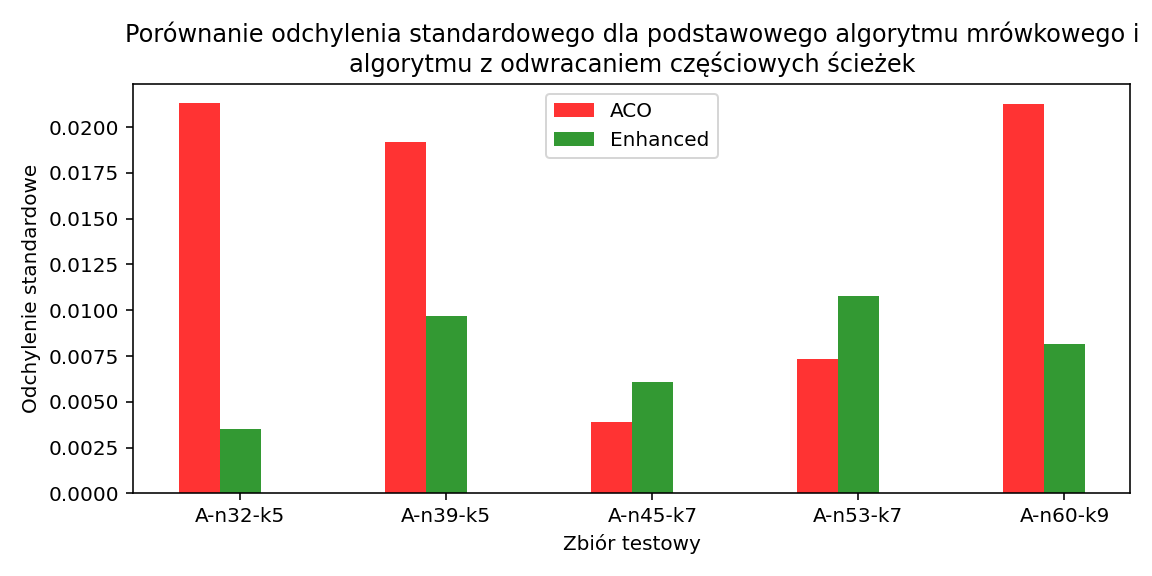
\includegraphics[width=0.75\textwidth]{deviation_enhanced.png}
    \caption{Porównanie odchylenia standardowego dla podstawowego algorytmu mrówkowego i rozszerzenia z odwracaniem częściowych ścieżek}
    \label{fig:deviation_enhanced}
\end{figure}

\subsection{Algorytm zachłanny wyznaczy ścieżkę szybciej niż dowolny algorytm mrówkowy, jednak będzie ona nieoptymalna}
Wynik: Hipoteza \textbf{potwierdzona}

W odróżnieniu od poprzednich algorytmów, w tym przypadku z oczywistych powodów pominięto analizę kolejnych iteracji oraz odchylenie standardowe wyników, skupiając się na podstawowych aspektach działania algorytmów takich jak jakość znalezionych wyników oraz czas działania.

Zgodnie z przewidywaniami, działanie algorytmu heurystycznego było wielokrotnie szybsze. Nawet dla największych testów wynik zwracany był po kilku milisekundach. W związku z tym, czasy działania przedstawione na rysunku \ref{fig:time_heuristic} są niezauważalne.

\begin{figure}[H]
    \centering
    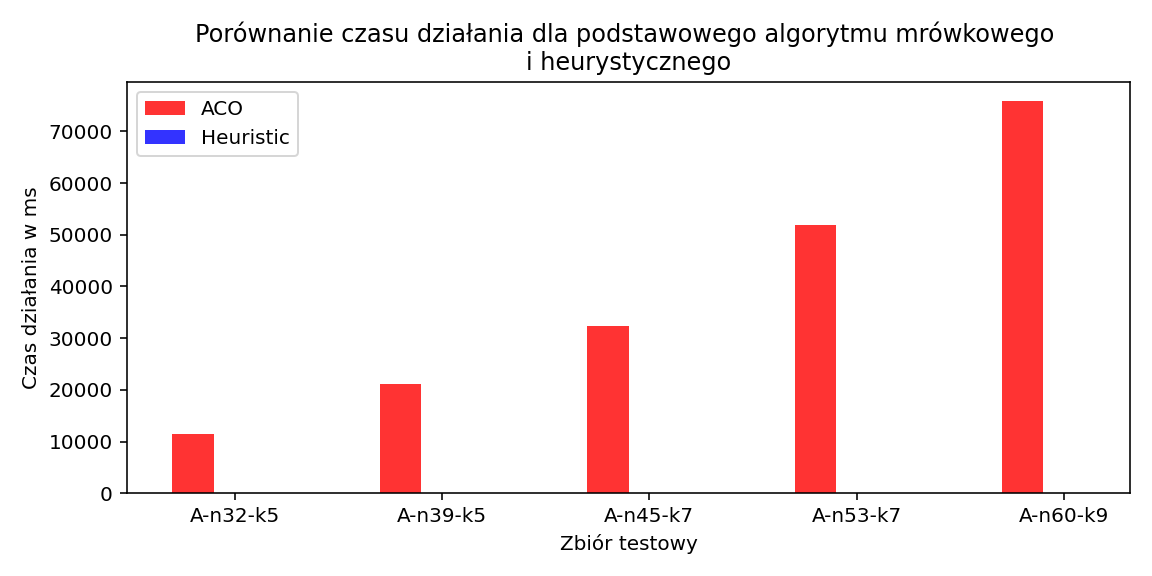
\includegraphics[width=0.75\textwidth]{time_heuristic.png}
    \caption{Porównanie czasu działania dla podstawowego algorytmu mrówkowego i algorytmu heurystycznego}
    \label{fig:time_heuristic}
\end{figure}

Również jakość zwróconego wyniku potwierdza przypuszczenia zawarte w hipotezie - we wszystkich przypadkach błąd względny był co najmniej dwukrotnie większy niż dla najprostszej wersji algorytmu mrówkowego, co obrazuje rysunek \ref{fig:errors_heuristic}

\begin{figure}[H]
    \centering
    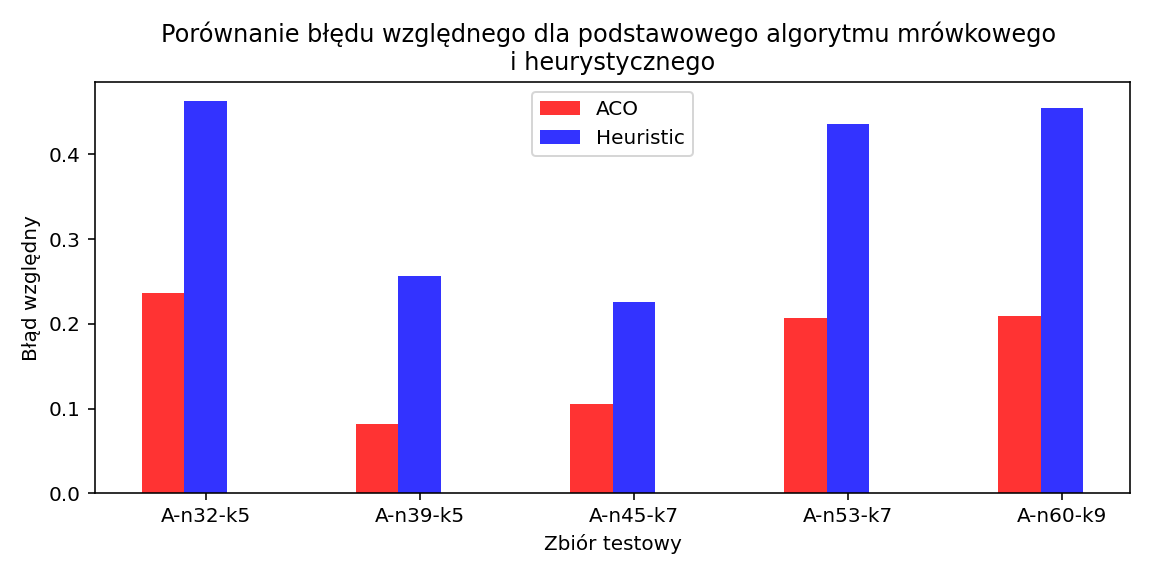
\includegraphics[width=0.75\textwidth]{errors_heuristic.png}
    \caption{Porównanie błędu względnego dla podstawowego algorytmu mrówkowego i algorytmu heurystycznego}
    \label{fig:errors_heuristic}
\end{figure}

\section{Wnioski}
Opisane w niniejszym raporcie wyniki badań różnych implementacji algorytmu mrówkowego do rozwiązania problemu CVRP potwierdzają użyteczność tego podejścia, jak również prezentują kilka niespodziewanych spostrzeżeń oraz kierunków dalszych badań. Najważniejszym wnioskiem jest jednak potwierdzenie wysokiej jakości rozwiązań uzyskiwanych za pomocą wszystkich trzech zaprezentowanych implementacji. Algorytmy te dają wyniki znacznie bliższe optymalnym, niż podejście heurystyczne, co potwierdza zestawienie na rysunku \ref{fig:errors_comparison}. 

\begin{figure}[H]
    \centering
    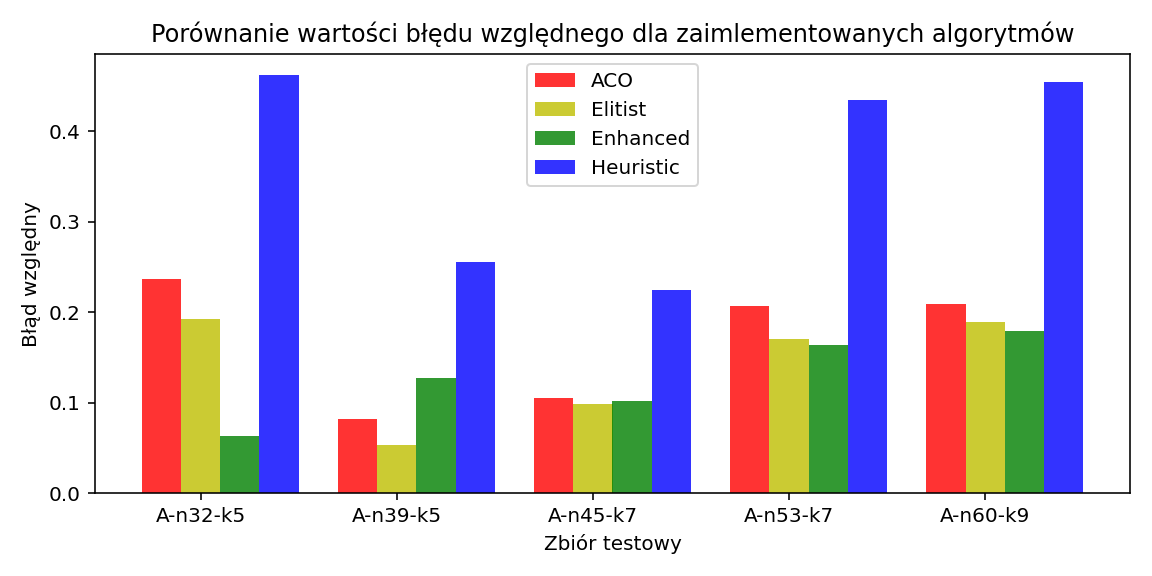
\includegraphics[width=0.75\textwidth]{errors_comparison.png}
    \caption{Porównanie błędu względnego dla zaimplementowanych algorytmów rozwiązywania CVRP}
    \label{fig:errors_comparison}
\end{figure}

Ponadto, obie przedstawione modyfikacje dają rezultaty lepsze niż podstawowa implementacja algorytmów mrówkowych, idąc jednak w dwóch różnych kierunkach:
\begin{itemize}
    \item Wprowadzenie mrówek elitarnych daje nieznaczną poprawę jakości rozwiązań bez dodatkowych nakładów czasowych.
    \item Odwracanie częściowych ścieżek w niektórych przypadkach znacznie poprawia jakość rozwiązania, jednak kosztem zwiększenia czasu działania o kilka/kilkanaście procent.
\end{itemize}

Mimo pozytywnych wyników, w trakcie badań pojawiło się również kilka kolejnych hipotez sugerujących potencjalne kolejne eksperymenty. Przede wszystkim dotyczą one powtarzalności wyników dla ulepszeń algorytmu mrówkowego przy różnych wartościach ziaren oraz zbiorów testowych. Kolejnym istotnym aspektem jest chociażby dobór optymalnych wartości parametrów dla różnych modyfikacji algorytmu. Prezentowane podejście korzystało z wartości parametrów wspólnych dla wszystkich implementacji, podczas gdy, wartości optymalne dla wersji podstawowej mogłyby się okazać dalekie od optymalnych dla kolejnych ulepszeń. Ciekawym aspektem może być również obserwacja wyniku ulepszonych wersji algorytmu mrówkowego (w szczególności algorytmu z odwracaniem ścieżek) dla większej liczby iteracji.

\printbibliography

\end{document}